\documentclass[11pt,a4paper]{article}
\usepackage{tikz} % for drawing figures
\usepackage{amsmath} % for equations
\usepackage{url} % for URLs
\usepackage{graphicx}
\usepackage{multicol}
\usepackage{varwidth}
\usepackage{blindtext}
\usepackage[pagewise, displaymath, mathlines]{lineno}
%\linenumbers
\usepackage{hyperref}
\usepackage{arydshln}

\usepackage{linguex} % ** special include in directory: for doing handy example labeling and bracketing
\renewcommand{\firstrefdash}{} % used for linguex package not to put hyphens in example refs (1a instead of 1-a)
%\usepackage{cogsci}
\usepackage{pslatex}
\usepackage{apacite}
\usepackage{placeins}
\usepackage{subcaption}

\newcommand{\sem}[1]{\mbox{$[\![$#1$]\!]$}}
\newcommand{\lam}{$\lambda$}
\newcommand{\gcs}[1]{\textcolor{blue}{[gcs: #1]}} 


% Possible title: Higher order pragmatic reasoning in reference games

%\title{On the purpose of ambiguous utterances}
\title{Learning about others:\\
	Pragmatic social inference \\ through ambiguity resolution
}
% OR: Pragmatic Social Inference while Observing Ambiguity Resolutions 
%                        and Strategically Generating Ambiguous Utterances
\author{
		Asya Achimova\\
		\href{mailto:asya.achimova@uni-tuebingen.de}{asya.achimova@uni-tuebingen.de}
	\and
		Gregory Scontras\\
		\href{mailto:g.scontras@uci.edu}{g.scontras@uci.edu}
	\and 
		Christian Stegemann-Philipps\\
		\href{mailto:christian.stegemann@uni-tuebingen.de}{christian.stegemann@uni-tuebingen.de}
	\and
		Johannes Lohmann\\
		\href{mailto:johannes.lohmann@uni-tuebingen.de}{johannes.lohmann@uni-tuebingen.de}
	\and
		Martin V. Butz \\
		\href{mailto:martin.butz@uni-tuebingen.de}{martin.butz@uni-tuebingen.de}
}

%our affiliations}


\begin{document}
\maketitle

\begin{abstract}

Bayesian accounts of social cognition successfully model the human ability to infer goals and intentions of others on the basis of their behavior. In this paper, we investigate whether we can extend this paradigm to communicative behavior, and explore whether ambiguity resolution provides socially-relevant information for the speaker about the mental states of the listener. Our main focus lies on the added information conversation partners may gain by observing each other resolve ambiguity. 
%computational modeling of the inference process within the Rational Speech Act framework.
%In particular, we asked whether ambiguity resolution may yield socially-relevant benefits, revealing parts of the privileged ground of the interpreter. 
In particular, we asked if speakers can (i) use response observations to infer unknown preferences of a listener, and (ii) strategically choose ambiguous utterances for learning about those preferences. 
%We ran experiments in a reference game framework and modeled the data with a Rational Speech Act model.
In a reference game experimental set up, we observed that
participants were able to infer listeners' preferences when analyzing their choice of objects given referential ambiguity.
Moreover, a subset of speakers were able to strategically choose ambiguous over unambiguous utterances in an epistemic, event-predictive, goal-directed manner, although a different group significantly preferred unambiguous utterances. 
We conclude that ambiguity resolution indeed reveals aspects of the knowledge, preferences, and beliefs of conversation partners, and that some of us are able to strategically use ambiguous utterances to gain knowledge about these aspects. 
                                                                 

\textbf{Keywords:} 
ambiguity; pragmatics; information gain; event-predictive cognition; Rational Speech Act models; social intelligence
\end{abstract}

\section{Ambiguity in natural language}

\noindent 
%Active inference---that is, the anticipatory, goal-directed, and epistemic invocation of behavior---is
%closely linked to the predictive mind perspective \cite{Friston:2015,Hohwy:2013,Clark:2016}. 
%The anticipatory nature of the human mind reveals itself in many domains.
%With respect to planning and executing manual sensorimotor interactions, 
%it has been shown that we anticipate future events and event boundaries, revealing anticipatory, event-predictive active inference processes \cite{belardinelli2016s, belardinelli2018mental,Friston:2015,Hayhoe:2003,lohmann2019hands}.
%Also in the language domain, active inference processes seem to continuously unfold \cite{Christiansen:2016}, compressing information into event-like units of thought \cite{Baldwin:2019tsi,Gaerdenfors:2014}.
%For example, neurophysiological data has shown that listeners predict the semantic category of upcoming words \cite{federmeier2002picture}.
%Moreover, the inference process takes the structural properties of sentences into account \cite{levy2008expectation}.
%Dynamic language models show that complex, event-predictive structures guide ambiguity resolution during comprehension and likely also constrain ambiguity generation during language production \cite{Elman:2019}. 

%When systematic abstractions become relevant, event-predictive biases seem to be at play, invoking the tendency to compress sensorimotor experiences, including language, into event-predictive encodings \cite{Baldwin:2019tsi,Butz:2016,Butz:2017a,DuBrow:2019tsi}.
%Various disciplines associated with cognitive science suggest that our minds develop event-compressed predictive encodings, which are recruited during decision making and action generation, including language production and comprehension, essentially determining thought itself in a highly active, epistemic, goal-directed manner  \cite{Baldwin:2019tsi,DuBrow:2019tsi,Elsner:2019tsi,Knott:2019tsi,Papafragou:2019tsi,Zacks:2019tsi}.
%Here, we reveal socially epistemic inferences and utterance productions in scenarios where we observe and actively generate social event-predictive interactions.


%On rare occasions, such communication failure can even be deadly: 
%\citeA{pinker2015sense} alludes to the Charge of the Light Brigade during the Crimean War as an example of a military disaster that was caused by vague orders.
%He also mentions how poor wording on a warning light was responsible for the nuclear meltdown at Three Mile Island. Finally, citing \citeA{cushing1994fatal}, Pinker describes how the deadliest plane crash in history resulted from pilots and air traffic controllers arriving at different interpretations of the phrase ``at takeoff''.

Ambiguity is ubiquitous during conversations: speakers rely on aspects of context and extra-linguistic reasoning to enrich the linguistic signal and deliver their intended meanings. Given that ambiguity can hinder the efficient transfer of information between conversation partners, it is not surprising that linguists have treated the possibility for ambiguity as a bug in the communication system \cite{chomsky2002minimalism} and suggested that ambiguity should generally be avoided \cite{grice1975}. If we look back at the study of ambiguity, we find that the strategy of ambiguity avoidance is much older than the pronouncements by modern linguists. Greek and Latin rhetoricians believed that a skillfully-written text allows for a perfectly accurate and lossless transmission of meaning to the reader or listener \cite{ossarichardson2019}; such a text avoids ambiguities.

The attitude toward ambiguity has at times been quite different in other disciplines, in part because the term itself can refer to multiple phenomena. For linguistic research, a word is ambiguous if it can have two separate meanings even in the absence of context, simply as a linguistic sign. In that sense, the word ``bat" is ambiguous between a winged mammal and a sporting implement. Ambiguity in the language system has been on the radars of philosophers starting with Aristotle \cite{sennet2016ambiguity}. 

In organizational communication---communication that aids production---ambiguity aligns closely with underspecification: an utterance is ambiguous when it does not provide every detail about the intended meaning, leaving room for the listener to interpret it. This freedom is important in communication between managers and their employees when managers set future goals that should stimulate rather than limit creativity \cite{mohr1983implications}. Ambiguity allows for the expression of ideas that are broadly true of a large group, as in company slogans or vision statements \cite{carmon2013}. There, the language needs to be general enough to allow every member of the team to relate those general goals to him- or herself. Similarly, ambiguous descriptions allow speakers to avoid conflict \cite{pascale1981art}: interlocutors find utterances that allow a range of interpretations and do not enforce a particular viewpoint. 

In the case of referential ambiguity, an ambiguous utterance may apply to several possible referents in a scene. Here we use the term `referential' in the sense of \citeA{frege1892sinn}, distinguishing the reference of a word---an object/property in the world---and its meaning. For example, a pronoun can be referentially ambiguous if there are multiple potential antecedents in the context. 
% \gcs{can we give citations for these various types of ambiguity?} 
It is this latter type of ambiguity that we focus on in this paper, although the lessons we learn are likely to apply to the broader range of ambiguity phenomena.

%Still, despite the teachings of classical philologists, authors continued to  create ambiguous texts and readers were faced with the challenge of interpreting them. The Bible is one of the most significant of such texts. In the sixteenth century, the Catholic church responded to the Reformation by proposing that the Bible can contain multiple meanings---\citeA{ossarichardson2019} equates these meanings with multiple paths that lead readers to God. In a sense, this proposal contained one of the first acknowledgments of the virtue of ambiguity, though with an important caveat: only God could introduce ambiguity, humans should not. 

%The search for efficient transmission of meaning has rested on an important assumption: we communicate to transfer knowledge to our conversation partner. It is the efficiency of this transfer that many recent experiments were designed to evaluate. To be more precise, communication was considered efficient if an experimental participant could follow instructions precisely. Yet, ordering actions and following instruction are probably not  the most common types of communicative acts \cite{foppa1995mutual}, and information-seeking might not be the only communicative task in which we engage \cite{markova1995preface}.
% \gcs{not sure what is meant by this last bit}. 

In spite of the early advice to avoid ambiguity, more recent research has begun to take notice of the efficiency ambiguity affords us: by relying on context to fill in missing information, we can reuse lightweight bits of language rather than fully specifying the intended message \cite{levinson2000,piantadosietal2012,wasow2015}. 
Viewed in this way, ambiguity serves as a feature---not a bug---of an efficient communication system.
This reasoning accords with years of psycholinguistic research documenting that speakers readily produce ambiguous utterances (see \citeNP{ferreira2008}, for an overview). 
Along related lines, \citeA{wasow2015} reviews a large body of evidence and concludes that ambiguity is rarely avoided, even in situations where its avoidance would be communicatively appropriate.
This observation stands at odds with the Gricean maxim to avoid ambiguity (\citeNP{grice1975}).
However, even \citeauthor{grice1975} recognized a case of strategic ambiguity where it could be the intention of the speaker to communicate more than one possible interpretation afforded by an ambiguous utterance. In such cases, recognition of the ambiguity serves as the communicative purpose of the utterance. \citeA{wasow2015}, on the other hand, reviews several cases where ambiguous production serves no obvious communicative purpose.


In the current work, we focus on the effects of resolving---or anticipating the resolution of---ambiguous utterances, identifying an additional benefit to ambiguous language: the \emph{extra} information we gain from observing how listeners resolve ambiguity.
We show that language users learn about each other's private knowledge (in Bayesian terms, their priors) when observing how ambiguity is resolved. 
When utterances leave room for interpretation, listeners must draw on their opinions, beliefs, and preferences to fill in the gaps;
by observing how it is that a listener fills in those gaps to resolve the ambiguity, speakers thus learn about the opinions, beliefs, and preferences of their conversation partner. 
Over the course of two studies, we first demonstrate that people are indeed able to infer hidden beliefs of their conversation partners on the basis of observed ambiguity phenomena; second, we show that some speakers can actively create situations of uncertainty, anticipating the epistemic value when observing the resolution of ambiguity. 
%we show how speakers update predictive models of listeners' preferences and beliefs when watching social event interactions, such as when offering a few objects to choose from and observing the object choice of the conversation partner. 
We thus show that humans can interpret the behavior of other people as driven by their motives, intentions, or personal characteristics---an idea that goes back conceptually to the attribution theory \cite{jones1965acts, kelley1967attribution, kelley1970social}.

To explain the behavior we observe in our experiments, we advance a computational cognitive model of the involved probabilistic inference processes formulated within the Bayesian Rational Speech Act modeling framework. 
%The main contributions of this paper are two-fold: 
%We formalize the human communicative behavior in a probabilistic Bayesian model, which approximates the dynamically unfolding reasoning processes, including limits thereof. 
While our model also pursues Bayesian inference, or ``psychological reasoning'', we do not focus on the inference of the actor's knowledge, that is, on \emph{learning from others} \cite{shafto2012learning}.
Rather, we focus on \emph{learning about others}, that is, learning about listeners' preferences when observing how they resolve ambiguity. 
We explore interpretive choices and the potential strategic, socially-epistemic usage of ambiguous utterances in anticipation of actors' responses. 
%To formalize our hypothesis, we adapt the Rational Speech Act model framework, modeling the underlying probabilistic interpretation processes and socially epistemic action choices. 
Interestingly, the modeling results reveal good interpretive abilities but also strong individual differences when the task is to choose (ambiguous) utterances strategically for gaining social knowledge. 

In what follows, we first provide computational background on referential ambiguity resolution (Section \ref{modelingTheory}).
In Section \ref{socialRSA}, we develop computational models that are able to infer the preferences of an agent that led her to a particular choice of objects, as well as a model that predicts which utterances are most useful to create the possibility of learning about the preferences of the conversation partner. 
Sections \ref{experiment1} and \ref{experiment2} give the results of the behavioral experiments, as well as an evaluation of modeling performance. 
Section \ref{discussion} concludes that participants were indeed able to use observable behavior of others to infer their prior beliefs, and hypothesizes why the ability to intentionally create epistemic situations can be found only in part of the population.


\section{Probabilistic modeling of ambiguity resolution} \label{modelingTheory}

%In search of the communicative purpose of ambiguous language, the current work identifies an additional benefit: the \emph{extra} information we gain from observing how listeners resolve ambiguity.
%We show that language users learn about each other's private knowledge when observing how ambiguity is resolved. 
%When utterances leave room for interpretation, listeners must draw on their opinions, beliefs, and preferences to fill in the gaps;
%by observing the concrete interpretation, speakers thus learn about the opinions, beliefs, and preferences of their conversation partner.
%As a result, in a naturalistic conversation, where speakers take turns, ambiguous utterances open interpretation spaces and the resulting interpretation choices dynamically and mutually reveal individual opinions, beliefs, and preferences. 


To see the potential epistemic benefit of ambiguous language, take the scenario in Figure \ref{FG-ref-game}.
Suppose a speaker produces the single-word utterance to signal one of the objects to a listener. Upon hearing ``blue,'' the listener faces referential ambiguity: the speaker could mean the blue square or the blue circle. 
Suppose further that, upon hearing ``blue'' in this scenario, the listener selects the blue circle.
In observing this choice, the speaker learns something about the private thoughts of the listener: what made her select the blue circle instead of the blue square? Perhaps the circle is more salient to the listener, or the listener has a preference for circles, or the listener may believe that the speaker has a preference for circles; there may even be mutual agreement that circles are to be preferred when possible. Importantly, by observing how the listener resolves the ambiguity in reference, the speaker can learn something about the private thoughts of the listener.


\begin{figure}
	\centering
	
\includegraphics[width=.5\linewidth]{images/rsascene-eps-converted-to.pdf}
	\caption{A simple reference game scenario from \protect\citeA{frankgoodman2012}.
		In the game, speakers are confronted with a collection of objects, which determine the current scenario $S$, where $S=\{solid\ blue\ square,\ solid\ blue\ circle,\ solid\ green\ square\}$ in the depicted example. 
		A speaker may choose a single-word utterance $u$ to signal one of the objects $s\in S$ to a listener.
		In the shown scenario, the following set of utterances is available: $U =\{\textit{``solid''},\ \textit{``blue''},\ \textit{``green''},\ \textit{``square''},\ \textit{``circle''}\}$.
		}
	% Martin: please leave in these details - this may appear slightly formal but very useful for the slightly more technical reader. 
	\label{FG-ref-game}
\end{figure}


However, accessing this added information requires the speaker to reason pragmatically about the pragmatic reasoning of the listener---a higher-order pragmatic reasoning.
In order to select a referent, the listener must first interpret the utterance. We follow \citeA{frankgoodman2012} in treating this interpretation process as active pragmatic, probabilistic reasoning: the listener interprets an utterance by reasoning about the process that generated it, namely the speaker, who selects an utterance by reasoning about how a listener would interpret it. \citeauthor{frankgoodman2012} model this recursive social reasoning between speakers and listeners, introducing the Rational Speech Act (RSA) modeling framework \cite{frankgoodman2012,frankejaeger2016,goodmanfrank2016}.

In this section, we first review  \citeauthor{frankgoodman2012}'s original formulation of RSA. We then explore recent work on social reasoning from a Bayesian perspective.

\subsection{Original RSA Formalization} \label{rsa}

\citeauthor{frankgoodman2012}'s RSA model of the reference game in Figure \ref{FG-ref-game} formalizes a state space, or scenario, $S$, as a particular set of objects. %(cf.~the example in Figure~\ref{FG-ref-game}). 
The model unfolds computations over the corresponding utterance space $U$, which consists of the set of possible utterances. %, which in turn contains all object features that are present in a particular scenario $S$.
At the base of the reasoning process, there is a hypothetical, na\"ive literal listener $L_0$, who hears an utterance $u\in U$ and attempts to infer the object $s \in S$ that $u$ is meant to reference. 
$L_0$ performs this inference by conditioning on the literal semantics of $u$, \sem{$u$}$(s)$, which returns $true$ (i.e., 1) for those objects that possess the uttered feature and $false$ (i.e., 0), otherwise.
As a result, object choice probabilities for the literal listener can be computed by: 
\begin{equation}
P_{L_{0}}(s\mid u) \propto \sem{$u$}(s),
\end{equation}
essentially returning a uniform distribution over those objects in $S$ that contain the uttered feature $u$.\footnote{Note that the context $S$ is typically not made explicit, but rather treated implicitly in the specification of the model.}


One layer up in the reasoning chain, the speaker $S_1$ observes the scenario $S$ and is assumed to have the intention to refer to a particular object $s \in S$.
$S_1$ chooses an utterance $u$ on the basis of its expected utility for signaling $s$ in the scenario $S$ to $L_0$, $U_{S_1}(u;s)$:\footnote{The original model in \citeA{frankgoodman2012} also includes a term for the utterance cost, $C(u)$. We ignore the term here since we assume uniform cost over all utterances.}
%which is determined by the log-likelihood of this particular object choice $U_{S_1}(u;s)$:
\begin{equation}
U_{S_{1}}(u;s) = \textrm{log}(P_{L_{0}}(s \mid u)).
\end{equation}
Depending on a ``greediness'' factor $\alpha$, the speaker chooses a particular utterance $u$ with a probability that is exponentially proportional to the utility estimate: 
\begin{equation}
P_{S_{1}} (u \mid s) \propto   \textrm{exp}(\alpha \cdot U_{S_{1}} (u;s)).
\end{equation}


At the top layer of the vanilla RSA model, the \emph{pragmatic} listener $L_1$ infers posteriors over $s$ on the basis of some observed utterance $u$.
However, unlike $L_0$, $L_1$ updates beliefs about the world by reasoning about the process that \emph{generated} $u$, namely the utterance choice of speaker $S_1$.
In other words, $L_1$ reasons about which object $s$ would have been most likely to lead $S_1$ to utter $u$ given the scenario $S$:
\begin{equation}
P_{L_{1}}(s \mid u) \propto P_{S_{1}}(u \mid s) \cdot P(s).
\end{equation}


\citeA{frankgoodman2012} tested the predictions of their RSA model against behavioral data from reference games as in Figure~\ref{FG-ref-game}.
To model production behavior (that is, which utterance should be chosen to communicate a given object), the authors used the probability distributions from $S_1$.
To model interpretation behavior (i.e., which object the speaker is trying to communicate on the basis of their utterance), the authors generated predictions from $L_1$.
\citeauthor{frankgoodman2012} found strong correllations between model predictions and behavioral data in both cases, confirming the validity of their model of pragmatic reasoning in reference games (see also \citeNP{qingfranke2015}, for a fuller exploration of the modeling choices).


\subsection{Bayesian Theory of Mind} \label{inferring}

While the RSA approach is aimed at inferring the meaning of an utterance by reasoning about the process that generated it, the inference process can also apply to aspects of the speaker's knowledge, or, in other words, her priors. This type of inference is crucial for social interactions, since it helps the conversation partners build more accurate anticipatory models of each others' behavrior. The anticipatory nature of human cognition has been registered in a number of cognitive domains \cite{Butz:2016, belardinelli2016s, belardinelli2018mental,Friston:2015,Hayhoe:2003,lohmann2019hands} and is viewed by some theoreticians as a core property of the human mind \cite{Clark:2016}. 

%In order to interact with the environment in an adaptive, versatile manner, we need to anticipate how objects and agents behave in that environment. 

Learning about the goals, beliefs, and preferences (i.e., the priors) of other agents depends on the ability of humans to infer hidden states by observing behavioral choices, thereby engaging in Theory-of-Mind reasoning. Our idea regarding the potential added utility of ambiguous language---that conversation partners can learn about each other as they observe ambiguity-resolution behavior---requires just this sort of reasoning. The large and growing literature on Bayesian Theory of Mind thus serves as inspiration for our own extended RSA model.

 The ability to infer others' preferences upon observing their behavioral choices develops early in childhood; \citeA{lucas2014child}, drawing from work in psychology and economics, formalize this process with a Mixed Multinomial Logit model which is driven by the assumption that, in making choices, agents maximize the subjective utility. \citeA{jara2016naive} review a large body of experimental work with children and adults, and propose a naive-utility-calculus model of so-called `commonsense psychology'---the ability of people to infer the hidden causes of others' behavior by treating them as utility-maximizing agents. 

%They argue that efficient learning is possible if we assume that agents' actions are driven either by physical (non-social) or communicative goals, but are crucially not random. The authors show that an observer can draw stronger inferences concerning an underlying hypothesis when the agent has a communicative goal. Their model predicts that learners use knowledge of agents' goals to evaluate how knowledgeable the agents are, and, as a consequence, how much a learner can trust the agents' actions to be informative about a hypothesis.

The process of mentalizing has been modeled within the Bayesian framework in a number of papers that look at the interpretation of the rational behavior of agents. \citeA{shafto2012learning} developed a Bayesian model of learning that formalizes the process of inferring others' knowledge about the world based on their actions and goals.
\citeA{evans2016learning} model the inference of prior preferences when agents are not fully consistent or have restricted knowledge about the choice options. The authors propose a model that can maintain uncertainty over the inferred beliefs. % and thus constitutes a more realistic inference model of human preferences---an essential step for building efficient Artificial Intelligence systems that can learn about the users. 
\citeA{baker2017rational} develop a computational model of Theory-of-Mind reasoning; %In their experiments, participants observed an agent moving through a complex landscape looking for her favorite food-truck. According to the setup, only two food trucks (Mexican, Lebanese, or Korean) are allowed to be on campus on any given day. Participants observe the movement of an agent among the food trucks present to interpret the agent's behavior and infer which food truck is her favorite, and whether she believes another food truck is hidden in a location that is out of line of sight of the agent currently. 
through a process of model comparison, the authors demonstrate that the inference crucially relies on joint reasoning about beliefs, desires, and percepts, since simpler models that rely only on a subset of these components are less accurate at predicting human judgments.
In a lexicon-learning paradigm, \citeA{woensdregt2016modelling} model how Bayesian inference about the beliefs of speakers can co-develop with the process of determining the likely referents of lexical items. The authors treat word learning as a process of inferring the intended meaning from hearing a word and observing the context in which that word was used. In a series of simulations, the model learns a lexicon and a perspective jointly; perspective in the model is defined as the salience of an object for the speaker, with salience inversely related to the distance between the speaker and the intended object. 
\citeauthor{woensdregt2016modelling}~further discuss what implications the ability to mentalize carries for reducing referential uncertainty and successful vocabulary learning.


%The utility-maximizing approach relies on a view of agents as inherently rational. 

Within the RSA framework, \citeA{degen2015wonky} show how inferring the hidden mental states of conversation partners can take the form of inferring priors. The authors explored how listeners infer the speaker's prior over world states when confronted with an utterance that conflicts with their own prior. If a listener hears that marbles were thrown into a pool and `some marbles sank', she infers that the likely prior over the world states (i.e., that marbles usually sink in water) is not shared by the speaker, thereby reasoning that the world must be `wonky'. In their model, listeners actively reason about a wonkiness parameter; in a wonky world, the listener switches from their informative prior to a uniform prior over the world states.
As another instance of Theory-of-Mind reasoning within the RSA framework, \citeA{yoon2018polite} model the comprehension of polite language that features so-called `white lies' (e.g., telling someone that their terrible cookies are `okay'). In the model, listeners jointly infer the state of the world (e.g., how good the cookies are) and the goals of the speaker (i.e., how much they prioritize politeness vs.~informativity).  
%utterances describing an assessment by inferring a prior distribution over conversation goals that include not only the aim to transfer information accurately but also social goals, such as appearing nice and letting the conversation partner save face. 
% Asya: I think we should mention Kao to show that we are aware of other RSA work that models the inference of mental states
In work on metaphorical language use \citeA{kao2014formalizing} also consider affective goals that justify non-literal interpretation of their utterances. The authors further model the comprehension of nonliteral language as a joint inference of the meaning of an utterance and an affective state of the speaker. %, showing an example of a Bayesian theory of mind modeling within the RSA framework.


%We further explore ambiguity use as a strategic tool that speakers may use to probe the listener to make an informative decision and reveal their preferences in a particular domain. Continuing the line of research, such as \citeA{yoon2018polite} and \citeA{kao2014formalizing}, we consider communication goals that go beyond pure information transfer. 


%section{Pragmatic social inference RSA model}
\section{Our model of social inference} \label{socialRSA}

Our work contributes to the broad literature on Bayesian Theory of Mind and more specifically to the modeling of prior inference in communicative settings within the RSA framework. Unlike previous papers that model the listener's inference over the priors of the pragmatic speaker $S_1$, we aim to model the inference process of a higher-order pragmatic speaker upon having observed a listener's ambiguity-resolution behavior. 

Our model builds on the vanilla version of RSA, modifying the listener's state prior $P(s)$ and enhancing the reasoning process towards a social component, yielding a {pragmatic social-inference RSA} model. %In that sense, the model belongs to the family of models known as uncertain RSA \cite{goodmanfrank2016}. 
By changing $P(s)$ to a non-uniform distribution, we model prior beliefs about which object the speaker is more likely to refer to, or, when viewed from a more self-centered perspective, which feature preferences $f$ the listener may have. 
For example, the listener may like blue things, such that she may be more likely to choose the blue square instead of the green one when hearing the utterance ``square'' in the scenario shown in Figure~\ref{FG-ref-game}.
As a result, when a pragmatic speaker produces utterance $u$ and observes the listener's referent choice $s$, the speaker may infer posteriors over possible feature preferences, attempting to explain the observed object choice in this way.

We use $L_0$ and $S_1$ from the vanilla model, but we now parameterize $L_1$'s state prior such that it operates given a feature preference $f$:
\begin{equation}
P_{L_{1}}(s\mid u,f) \propto P_{S_{1}}(u \mid s) \cdot P(s \mid f).
\end{equation}
We then model a pragmatic speaker $S_2$, who updates beliefs about $L_1$'s preferences, $P(f)$.
$S_2$ observes $L_1$'s choice of $s$ given the produced utterance $u$ and then reasons about the likely feature preference $f$ that $L_1$ used to make the observed choice:
\begin{equation}
P_{S_{2}}(f\mid u,s) \propto P_{L_{1}}(s \mid u,f) \cdot P(f).
\end{equation}


We also model the reasoning process by which a speaker may select the best utterance to learn about the preferences of the listener, essentially striving to maximize expected information gain concerning the listener's feature preferences.
Starting with no knowledge of the listener's preferences, $S_2$ can be assumed to expect a uniform (i.e., flat) feature preference prior $P(f)$.
The more the speaker's posterior beliefs about the preferences, $P_{S_{2}}(f\mid u,s)$, deviate from the uniform prior, the more the speaker will have learned about the listener's preferences. 
We can thus model this reasoning in light of expected information gain, which can be equated with the attempt to maximize the KL (Kullback-Leibler) divergence between the speaker's flat prior and the expected posterior over the listener's feature preferences $f$, integrating over all hypothetically possible object choices $s \in S$: %\gcs{can we assume a uniform cost and then remove $C(u)$ from our equations, mentioning this move in a footnote?}
\begin{equation}
P_{S_2}(u) \propto \sum_{s:\  [\![u]\!](s)=1} P_{L_1}(s|u,f)\ \exp(\lambda \cdot \textrm{KL}(P(f)\mid\mid P_{S_{2}}(f\mid u,s))),
\label{eq:kldivlambda}
\end{equation}
where the factor $\lambda$ scales the importance of the KL divergence term. 


We evaluate two versions of the model. 
The full models assumes the recursive reasoning process integrating the full RSA formalism.  
The full model thus assumes that feature-preference inference not only considers the current object choices possible, but also differentiates the choice options further with respect to their pragmatic plausibility. 
For example, the full model captures the fact that when a speaker utters ``blue'' in the object situation depicted in the example shown in Figure~\ref{FG-ref-game} and has the intention to refer to one particular object, she is more likely to refer to the blue square than to the blue circle, because in the latter case the utterance choice ``circle'' would have been unambiguous and thus a better utterance choice.

Recently, it has been shown that even in the original, simpler reference games, fewer layers of reasoning often perform equally well or better than more complex RSA-based models \cite{sikos2019}.
Accordingly, our simple model removes the reasoning about alternative utterances and allows the pragmatic speaker to directly tap into the (expected) interpretation of $L_0$, augmenting the literal listener's choice likelihoods with the feature-preference-dependent object prior $P(s\mid f)$:
\begin{equation}
P_{L_{0\textrm{-simp}}}(s\mid u,f) \propto \sem{$u$}(s) \cdot P(s\mid f).
\end{equation}

The pragmatic speaker $S_{1\textrm{-simp}}$ then reasons directly about the modified literal listener $L_{0\textrm{-simp}}$: 
\begin{equation}
P_{S_{1\textrm{-simp}}}(f\mid u,s) \propto P_{L_{0\textrm{-simp}}}(s\mid u,f) \cdot P(f).
\end{equation}

As a result, the simple model ignores any indirect pragmatic reasoning considerations about which object the speaker may refer to given an utterance and a particular object constellation.
The model simply assumes that all objects may be chosen that match the utterance semantics, modifying these choice options depending on the state prior that incorporates feature preferences. The corresponding utterance-selection model simplifies the reasoning process accordingly:
\begin{equation}
P_{S_1\textrm{-simp}}(u) \propto \sum_{s:\  [\![u]\!](s)=1} P_{L_0}(s|u,f)\ \exp(\lambda \cdot \textrm{KL}(P(f)\mid\mid P_{S_{1\textrm{-simp}}}(f\mid u,s))).
\label{eq:kldivlambdasimp}
\end{equation}

In evaluating our model predictions below, we compare the modeling performance of the full model with that of the simple model.

%\section*{Methods}

\section{Experiment 1: Inferring preferences} \label{experiment1}

Our first task is to check the inferences of the pragmatic speaker having observed that a listener selects some object $s$ in response to an utterance $u$. 
Is it possible to draw inferences about the most likely preferences the listener had when making her choice? 
Can this inference process be modeled by our RSA model---that is, by recursive Bayesian inference?
%A sample trial is shown in Figure~\ref{exp1-trial}.



\subsection{Participants}

We recruited 90 participants with US IP addresses through Amazon.com's Mechanical Turk crowdsourcing service. Participants were compensated for their participation. On the basis of a post-test demographics questionnaire, we identified 82 participants as native speakers of English; their data were included in the analyses reported below. We obtained a confirmation from all the participants that they agreed to participate in the study.

\subsection{Design and methods}

We presented participants with a series of reference game scenarios modeled after Figure~\ref{FG-ref-game} from \citeA{frankgoodman2012}.
Each scenario featured two people and three objects.
One of the people served as the speaker, and the other served as the listener. The speaker asks the listener to choose one of the objects, but in doing so she is allowed to mention only one of the features of the target object. Participants were told that the listener might have a preference for certain object features, and participants were tasked with inferring those preferences after observing the speaker's utterance and listener's object choice. A sample trial is shown in Figure~\ref{exp1-trial}.

\begin{figure*}[ht]
	\centering
	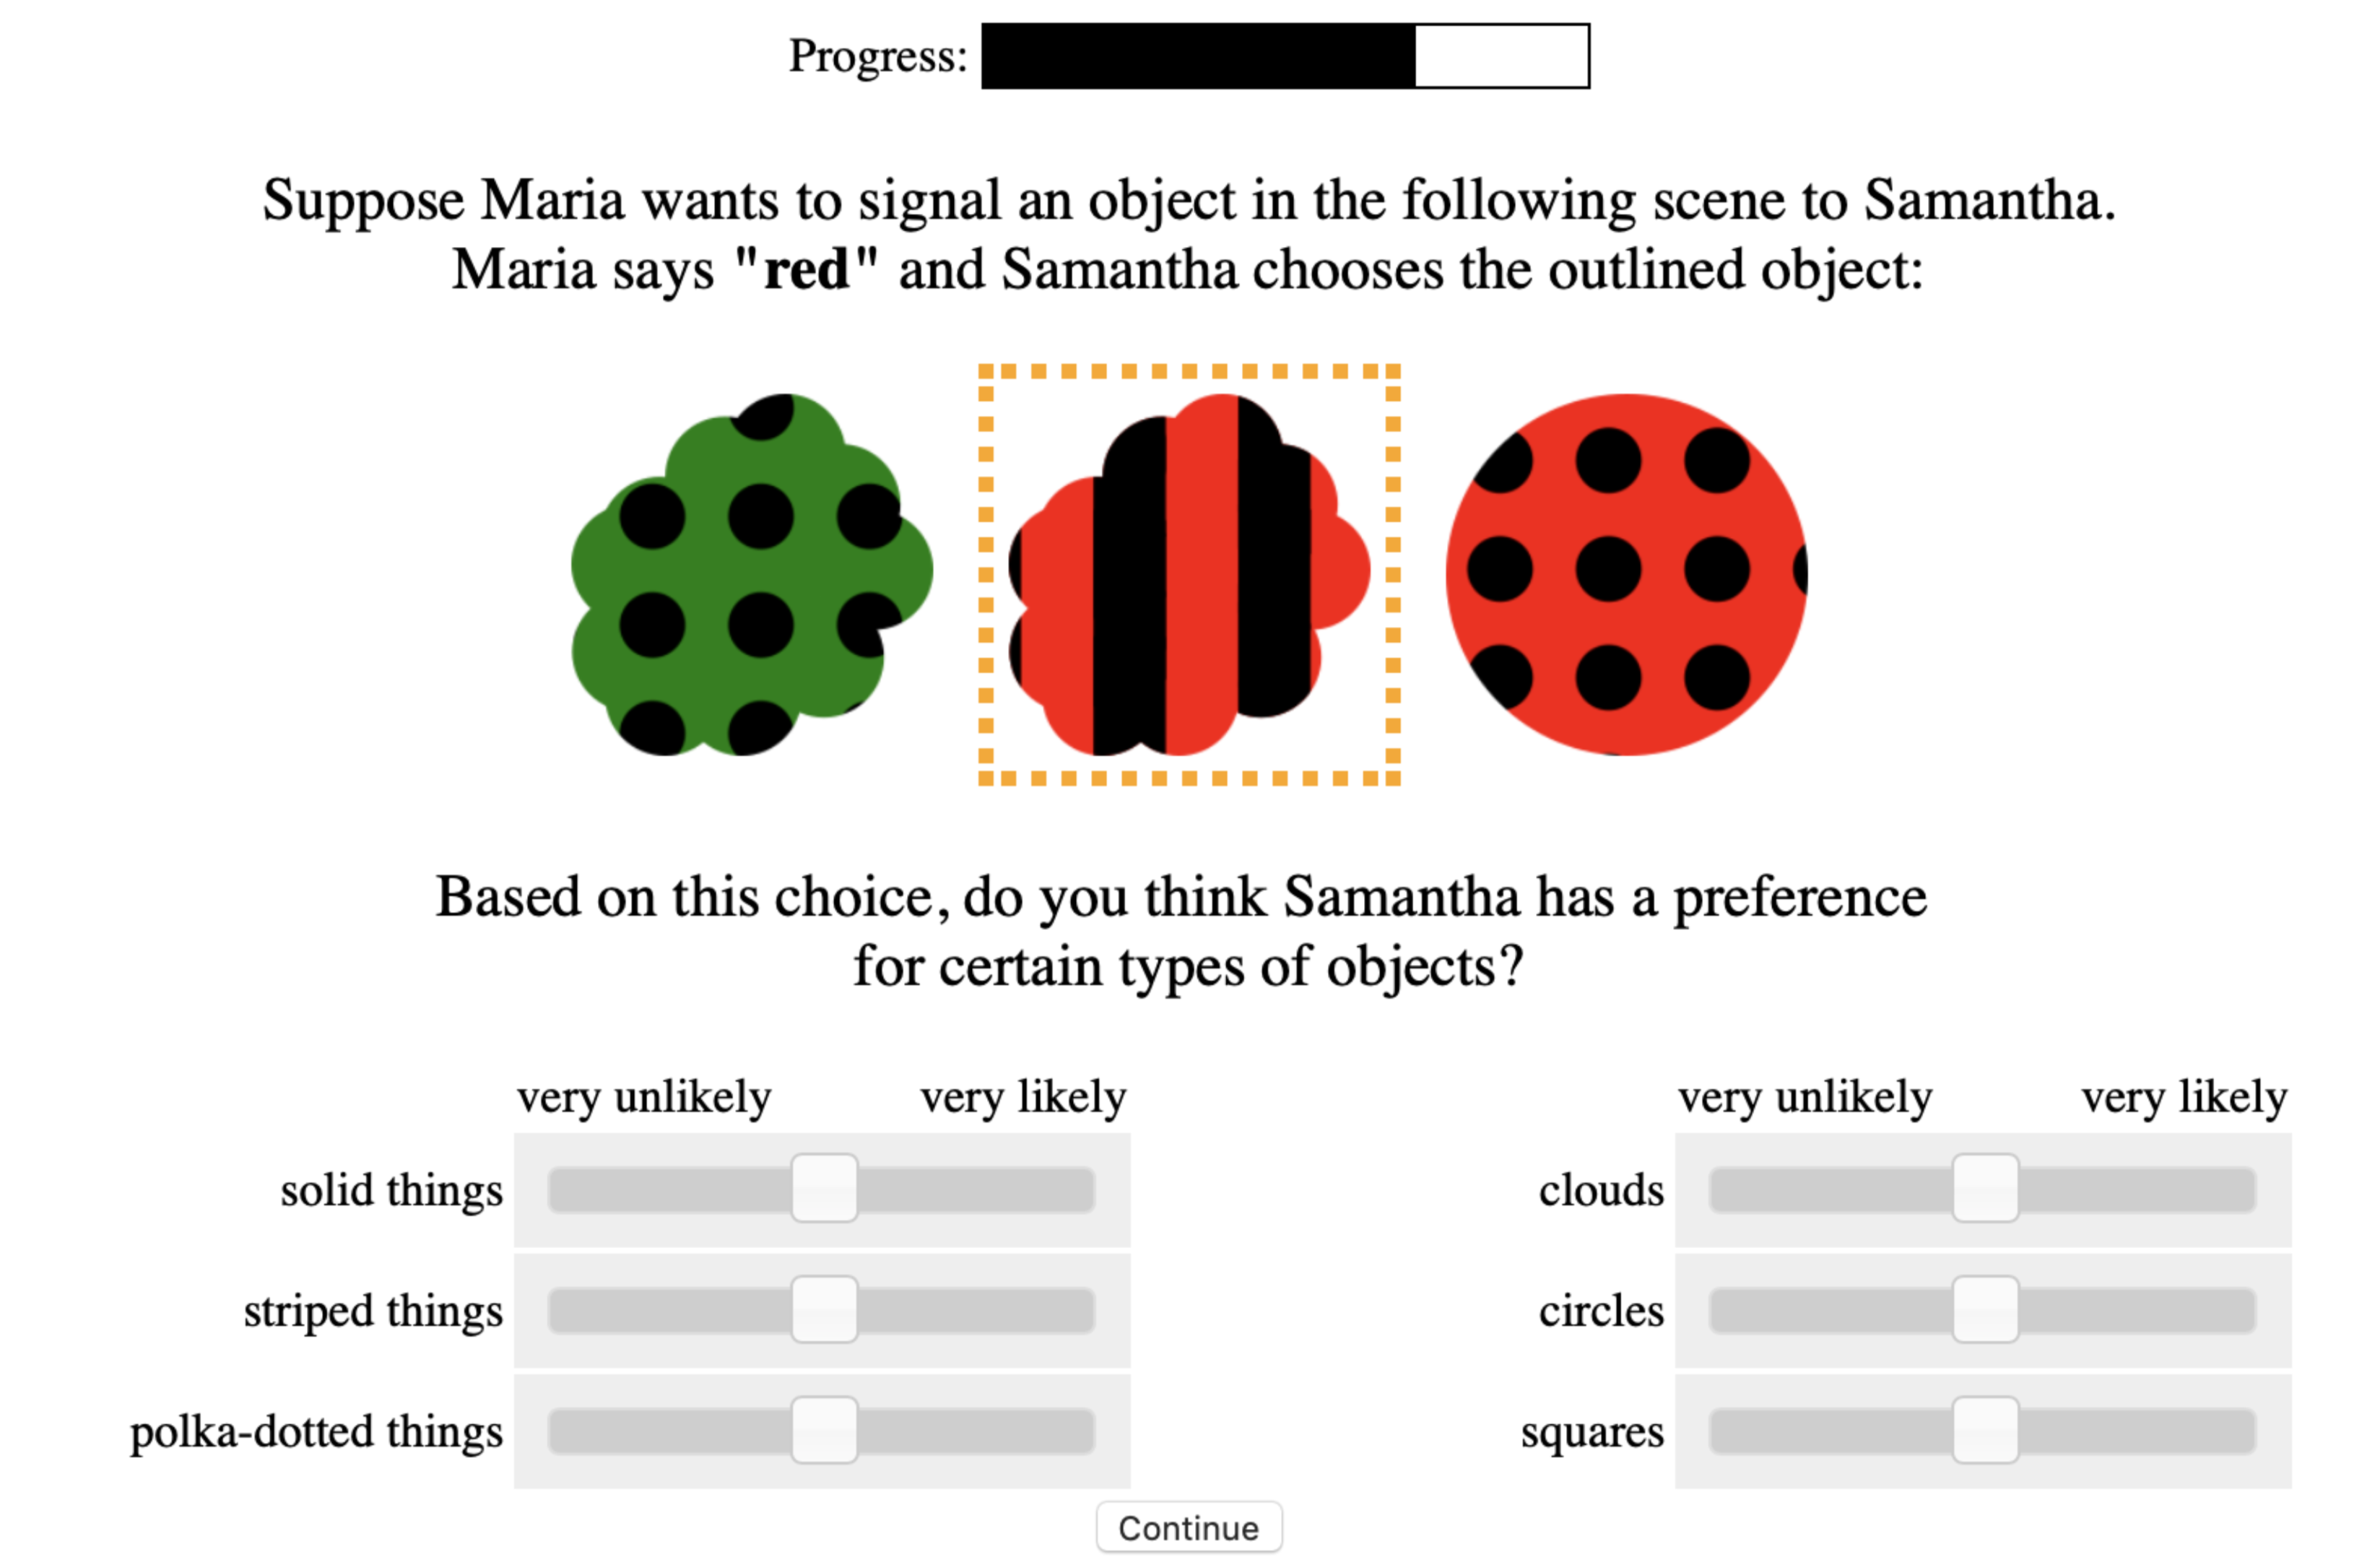
\includegraphics[width=4.5in]{images/preference-trial.png}
	\caption{ \small{A sample trial from \emph{Experiment 1: Inferring preferences}. Each trial portrays a speaker and a listener. The speaker produces an utterance to refer to one of the objects. The listener picks the object with the orange-dotted outline. Participants were tasked with evaluating what preferences of the listener may have led her to the particular object choice, specifying their inference by adjusting the sliders for each of the features}.}
	\label{exp1-trial}
\end{figure*}

We followed \citeA{frankgoodman2012} in our stimuli creation. Objects were allowed to vary along three dimensions: color (blue, red, green), shape (cloud, circle, square), and pattern (solid, striped, polka-dotted). The speaker's utterance was chosen at random from the properties of the three objects present, and the listener's choice was chosen at random from the subset of the three objects that possessed the uttered feature. By varying the object properties, the targeted object, and the utterance, we generated a total of 2400 scenes. Speaker and listener names were chosen randomly in each trial. Participants saw the speaker's utterance in bold (e.g., ``red'' in Figure \ref{exp1-trial}) and the listener's choice appeared with a dotted orange outline (e.g., the center object in Figure \ref{exp1-trial}). Based on the observed choice, participants were instructed to adjust a series of six sliders to indicate how likely it is that the listener had a preference for a given feature. The sliders specified the six feature values of the two feature dimensions that were not mentioned in the speaker's utterance (e.g., pattern and shape in Figure \ref{exp1-trial}). 

To compare our model's predictions to the human data, we calculated an average value for each slider.
%, binning data into 48 ambiguity classes.
% for Experiment 1 and 14 classes for Experiment 2. 
We excluded the sliders if their corresponding feature value was not present in a scene. For example, for the trial depicted in Figure \ref{exp1-trial}, we excluded the sliders for solid things and squares since none of these are present, and therefore no learning about them is possible.

To determine model correlations with the gathered data, we partitioned the data into ambiguity classes, similar to \citeA{frankgoodman2012}. Depending on how many features competitor objects share with the chosen object, we were able to identify 48 ambiguity classes, which group the constellations that have the exact same ambiguity pattern. The ambiguity classes identified in Experiment 1 distinguish how many objects are referenced by the utterance, how the referenced objects differ in their two non-uttered features, and how the non-referenced objects differ from the referenced objects and from each other.
As a result, each ambiguity class yields unique model predictions for the individual features present (with respect to their ``ambiguity role'' in the particular ambiguity class) in corresponding scenarios $S$, effectively distinguishing all model-relevant cases. Please see the Appendix for examples of different classes.


%For example, considering the top-left-most case, ,where the utterance ``red" refers to two possible objects and the choice falls onto one of them (here the red cloud), which shares one property with the other, not referenced object (its cloud shape), but no further properties with the other referenced object (neither its shape nor its pattern). Thus, its other property is unique (its striped pattern)
%If, as an alternative scenario, he utterance was ``green", only one object would qualify (the green, dotted cloud), preventing the learning about preferences. 
%In that case, the model would assign equal probability to the listener's preferring dotted objects, striped objects, clouds, and squares. 
%Once the model establishes that more than one object can be picked, it also needs to consider whether alternative objects share their features with the target object. For example, if both red objects were also striped, the model would not be able to infer any preferences about the pattern. 
%In addition to these considerations, ambiguity classes also distinguish whether the objects that are not referenced by the utterance share any of their feature values.

Participants completed a series of fifteen trials. Objects and utterances were chosen as detailed above, with the constraint that ten trials were potentially informative with respect to listener preferences and five trials were uninformative with respect to listener preferences (e.g., observing that the listener chose one of three identical objects). 

\subsection{Free parameters and optimization procedure}


%We binned those scene types 
%For all scene types, the actual feature values and objects in a scene were reordered according to the specific preference inference involved \gcs{I'm not sure what you mean here}. 
%Thus, after reordering, the results of the individual slider values for individual scenes in each scene type could be averaged for both the participant data and the model predictions. 

We fit the model parameters either at the individual level or at the group level by optimizing the KL divergence between the data and the model predictions:

\begin{equation}
	\textrm{KL}(P_{data}(f \mid u,s)\mid\mid P_{model}(f\mid u,s)),
\end{equation}

\noindent where $P_{data}(f\mid u,s)$ specifies a participant's normalized slider-value setting, which offers empirical estimates of the feature-preference posterior given object scene $S$, a particular utterance choice $u$, and the consequent object choice $s$;
$P_{model}(f\mid u,s)$ specifies the corresponding model posterior, either $P_{S_{2}}(f\mid u,s)$ in the case of the full model or $P_{S_{1\textrm{-simp}}}(f\mid u,s)$ in the case of the simple model. 
%Since no conclusions can be drawn concerning feature values that are not present in the scene, we ignored the respective feature preference estimates.
By minimizing the summed KL divergence between the empirical and model-predicted preference posteriors over all considered trials, we maximize the model fit to the participants' data. 
Moreover, we can use the minimized KL divergence values to calculate the $G^2$-statistic and perform the likelihood-ratio test for nested models, since $G^2$ values are approximately chi-square distributed \cite{Lewandowsky:2011}. 
Individual vs.~global parameter fitting allows us to explore potential differences between participants.
In the case of individual model parameter optimization, parameters were optimized for each individual participant separately, determining the KL divergence with respect to the participant-specific set of trials. 
In the case of global optimization, all trials of all participants were used to determine the summed KL divergence.
% Martin: I find this point confusing and not quite correct: 
%%  and, more importantly, to evaluate whether the Gricean reasoning strategies apply at the level of individual speakers or only to the population as a whole \cite{franke2016reasoning}. 

We fit three parameters for our full model and two for the simple model.
%We hypothesized that participants may either go through all the layers of pragmatic reasoning, and additionally calculate the preferences that lead to particular object choice. The last layer of this model $S_2$ returns a posterior distribution over inferred feature preferences $f$ after observing a listener selecting an object in response to an utterance. 
%In a simpler model, the object choice is driven only by a $L_0$ semantics enhanced with priors over feature preferences. Upon hearing an utterance \textit{blue} a participants assigns equal probabilities to all blue objects in a scene, and the actual choice of object signals a preference of other feature values that object has. For example, picking a blue circle rather than a blue square is driven by a prefrence for circles.
The soft-max scaling factor $\alpha$ is only relevant for the full model; it  controls how likely speaker $S_1$ is to maximize utility when choosing utterances. 
The default value is typically set to $\alpha=1$ (i.e., no scaling). 


The softness parameter $\gamma$ regulates the strength of individual feature preferences $f$:
\begin{equation}
	P(s \mid f) \propto \begin{cases}
		1 + \gamma, & \text{if}\ s\ \text{contains}\ f \\
		\gamma, & \text{otherwise}
	\end{cases},
\end{equation}
controlling the choice probability of those objects $s$ that contain feature $f$ compared to those that do not.  
A value of $\gamma=0$ models a hard preference choice; in this case, the speaker always chooses one of the preferred objects. 
On the other hand, when $\gamma \rightarrow \infty$, the choice prior becomes uniform over all objects, thus ignoring feature preferences. 
% That is, a large value of $\gamma$ approximates uniform prior feature preferences.
% I tried to write it in a more general form that works for both P = 0 and P = 1 but I'm not sure that works.
% This is the R code:
%objectPreferenceSoftPriors[[utt]] <- objectPreferenceHardPriors[[utt]] + softAddProb
%objectPreferenceSoftPriors[[utt]] <- objectPreferenceSoftPriors[[utt]] / sum(objectPreferenceSoftPriors[[utt]])
%$$ P(s_{\textrm{cloud}}\mid f_{\textrm{cloud}}) = \frac{1 + \gamma}{1 + 3\gamma}
%%\end{equation}
% This is what we wrote. It makes sense for P = 1 but I'm not sure the numbers come out right when we calculate how softness changes the probability of objects that don't qualify.
For example, in the trial shown in Figure~\ref{exp1-trial}, there are two objects that match the utterance $u=\text{``red''}$: a red striped cloud and a red dotted circle.
When $\gamma=1$, $P(s_{\textrm{red\ striped\ cloud}}\mid f_{\textrm{``cloud''}}) = 2/3$, while
$P(s_{\textrm{red\ dotted\ circle}}\mid f_{\textrm{``cloud''}})= 1/3$, yielding a soft preference for clouds.
% The softness parameter $\gamma$ regulates the probability that the middle object will be picked if a person has a preference for clouds. 
%Preference softness increases with $\gamma$: 
%a value of $\gamma=0$ specifies a hard preference, which means that the listener will always choose the object that holds the preferred feature value if possible (e.g., clouds when clouds are preferred). 
We use $\gamma=0$---that is, hard preferences---as the default model value.
%Let us see how the probability changes if $\gamma$ is set to 0.2:
% $$ P(s_{\textrm{cloud}}\mid f_{\textrm{cloud}}) = \frac{1 + 0.2}{1 + 3 \cdot 0.2} = 0.75
%%\end{equation}

%Here the preference becomes softer: a subject will pick up clouds with a probability of 0.75 rather than 1.
%On the other hand, $\gamma \rightarrow \infty$ specifies a uniform feature value preference, or no actual preference. 

%The softness parameter $\gamma$ determines how strong a preference is if a certain feature value is indeed preferred.
%such that the RSA models can be viewed as being nested within the default model.
% Note: I removed $\beta$ because it complicates things enormously and proved to be not really relevant.

Finally, we allow for the possibility of noise in our human data introduced by participants not following instructions.
Parameter $\beta$ models the possibility that listeners choose objects that do not pass the semantic filter of the literal listener, allowing for non-literal interpretations that result in choosing objects whose features do not match the received utterance $u$. 
The computation is equivalent to the softness parameter above, in this case softening the object choices of the literal listener $L_0$ towards a uniform choice over all objects present. 
%$$ P(s_{\textrm{x}}\mid u_{\textrm{x}}) = \frac{P(s\mid u) + \beta}{\sum P(s\mid u) + 3\beta}
%%\end{equation}
Again, $\beta=0$ models a hard object choice---that is, full obedience to the uttered instruction $u$---while $\beta \rightarrow \infty$ models a uniform object choice---that is, full ignorance of $u$. 

The effect of this parameter being higher than the default value of $0$ is visible when the properties of objects that do not qualify as a possible referent given an utterance (for example, blue objects when the speaker said `red') affect the slider values. Consider a scene containing three objects: a red square, a red circle and a blue cloud. If the listener picks the red square following the utterance 'red' and rejects the red circle, the subject is expected to indicate that the listener likes squares and does not like circles. Since there are no red clouds in that scene, the slider for clouds cannot be adjusted to an informative value. However, if the obedience parameter $\beta$ is above $0$, the modeled participant would lower the slider for clouds, since a cloud was not chosen (despite the fact that the blue cloud did not qualify as a potential referent).
This parameter allows the model to capture noise associated with adjusting sliders when no explicit evidence for updating a particular type of preference was actually present in the scene.
%As $\beta$ increases, speakers disregard instructions and assign non-zero probabilities to objects that do not correspond to the utterance; with $\beta = 0$, speakers fully obey the instructions and only consider objects with the named property (e.g., only red objects following the utterance \textit{red}).

\subsection{Results}
\subsubsection{Models with global optimization}

%We fit the following free parameters to optimize the predictions of the models. First, the full model includes a ``greediness'' parameter $\alpha$ that controls how likely it is that speakers choose the best-suited utterance to signal a particular object to a listener. This parameter is absent in the simple model since it relies on fewer layers of reasoning. The second parameter $\gamma$ controls how soft the preferences are. Hard preferences enforce the choice of the preferred object type, while increasing softness converges towards no object preference. Similarly, the obedience parameter $\beta$ allows subjects to choose objects that do not qualify for the utterance. As for the preference parameter $\gamma$, the $\beta$ range includes hard obedience on the one side of the spectrum -- for example, definitely choosing a blue object when hearing ``blue'' -- and full ignorance of the utterance at the other extreme, choosing uniformly from all available objects. 
%the , for example, subjects will consider objects that are not blue upon hearing ``blue''.


% We first present results for the globally-optimized versions of  PSIRSA .
% I used the code length(levels(as.factor(uniqueCCode))) to calculate the number of conditions
%Since not all of the stimuli allowed for inference of preferences in the same way, we introduced a new categorization of stimuli. Our base model would then predict the same preferences for the same category of stimuli. The categorization takes into account the distribution of features, the chosen object and which feature was uttered. Each category consists of 3 tuples of 2 digits. Each tuple refers to one feature, where the first tuple always refers to the uttered feature. The first digit in each tuple would then denote how many objects share the value of the picked object for the corresponding feature. In figure \ref{FG-ref-game}, if the utterance was blue and the blue square was picked, the first tuple would reference color and its first digit would be a "2". Note that this does not determine which other object shares the feature value, i.e. "blue". To compensate, the second digit of the tuple denotes which other object shares this value. This depends on the order of the objects---we stipulated that the picked object would be the first. The further order would be determined by which other object shares this specific value, i.e. the "blue circle" in figure \ref{FG-ref-game} would be the first of the "other objects" and the "green square" the second. The picked object is at position zero in this sense. Thus the first tuple for figure \ref{FG-ref-game} would be (2,1). For the other tuples, the first digits would be "2" for shape and "3" for texture. To streamline the category code we stipulated that we would order the features in descending order of their first digit, so that we would have texture's "3" next in figure \ref{FG-ref-game}. If a tuple starts with "3" or "1", the second digit would simply denote whether the other objects have different values for that feature or the same. Thus we would have (3,2) for texture, with the second digit signaling that the non-picked objects share their texture. The tuple for shape would finally be (2,2), because the value "square" is shared with the second other object (see above). Thus for figure \ref{FG-ref-game} we would end up with [(2,1),(3,2),(2,2)].
Linear regression analysis was used to test whether the model values predicted the human data. 
As Table \ref{global} shows, the full and simple models with softness ($\gamma$) optimized globally provide nearly identically-good fits to the data (full: $r^2 = 0.86$; simple: $r^2 =  0.86$).\footnote{Here and throughout the paper we report adjusted $r^2$ values. All results were significant at the $p < 0.001$ level if not stated differently in the text.}
%Figure~\ref{simple-global-and-cross-validated} \gcs{this isn't what the figure shows}). 
% Asya: true! sorry about the mistake! I think we took out some of the figures, the refernce was wrong
%The simple model yields a value of $r^2 = 0.8607$ when only softness parameter $\gamma$ is optimized ($\gamma=0.2204$ after optimization). 
The simple model with both parameters optimized globally captures nearly all of the variance in the human data ($r^2 = 0.98$); in this model, the obedience parameter $\beta$ is estimated at $0.27$ after optimization, indicating that participants indeed considered (possibly subconsciously) the option to interpret utterances non-literally. 
% only $\gamma$ optimized: Multiple R-squared:  0.8614; gamma=0.220358
% $\gamma$ and $\beta$ optimized: Multiple R-squared:  0.9789; gamma=0.2210127, beta=0.2692707
%The full model yields nearly identical values.
%When optimizing only the softness parameter $\gamma$, a value of $r^2 = 0.8568$ ($F(1, 190) = 1144$) is reached ($\gamma=0.2231$)
The full model with both $\alpha$ and $\gamma$ optimized performs slightly better than the version with only $\gamma$ optimized ($r^2 = 0.86$).
% ($F(1, 190) = 1144$) is reached ($\alpha=0.1797$, $\gamma=0.2205$).
When optimizing all three parameters, the full model performs markedly better ($r^2 = 0.98$), on a par with the simple model with both parameters optimized. % ($F(1, 190) = 8170$) ($\alpha=0.2657$, $\gamma=0.2214$, $\beta=0.0030$).
%, not quite reaching the correlation of simplePSIRSA, which may be due to some subtle interactions between parameters $\alpha$ and $\beta$. 
% only $\gamma$ optimized: Multiple R-squared:  0.8576 ; gamma=0.2231055
% only $\alpha$ and $\gamma$ optimized: Multiple R-squared:  0.8614; alpha=0.1797266, gamma=0.2204913
% all three parameters globally optimized: Multiple R-squared:  0.9773; alpha=0.26568, gamma=0.2214308, beta = 0.003027947\\

\begin{table}[t]
\begin{tabular}{p{3.5cm}cccccc}
	\hline
	Model & $r^2$ & $df$ & $F$ & Soft. $\gamma$ & Obed. $\beta$ & Util. $\alpha$ \\
	\hline

	\hspace{1cm}\textit{Simple model} & & & & & \\
	
	Softness $\gamma$ & 0.8607 & 1,190 & 1181 & 0.2204 & & \\
	Softness $\gamma$ \& Obedience $\beta$ & 0.9788 & 1,190 & 8823 & 0.2210 & 0.2693 & \\
	
	\hspace{1cm}\textit{Full model} & & & & & \\

	Softness $\gamma$ & 0.8568 & 1,190 & 1144 & 0.2231 & & \\
	Softness $\gamma$ \& Utility $\alpha$ & 0.8607 & 1,190 & 1144 & 0.2205 &  & 0.1797\\
	Softness $\gamma$ \& Utility $\alpha$ \& Obedience $\beta$ & 0.9772 & 1,190 & 8170 & 0.2214 & 0.0030 & 0.2657\\
	\hline
\end{tabular}
\caption{Optimization summary (global) for Experiment 1 model predictions.}
\label{global}
\end{table}

Overall, the models accurately capture the participants' inferences over the feature preferences that lead to the choice of an object. %, and, notably, simplePSIRSA models this inference process very well.
Moreover, the greater complexity and added flexibility of the full model (controlled by the added parameter $\alpha$) does not yield any modeling improvement, implying that performance in our task can be modeled as more shallow a reasoning process within the simple model.
%modeled by the simple model typically unfolded in the minds of the participants.  

% \footnote{We were unable to perform a likelihood ratio test to compare these models since they are not nested.}



\begin{figure}[ht]
	\centering
	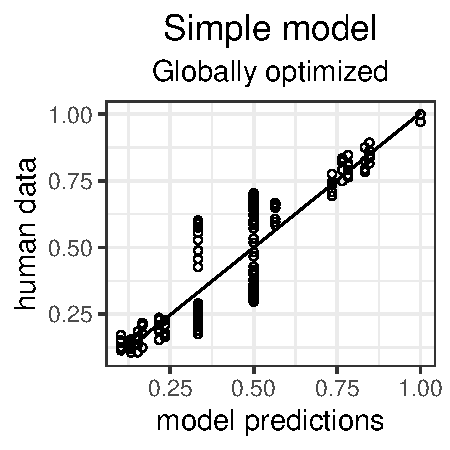
\includegraphics[width=2in]{images/m13.pdf}
%	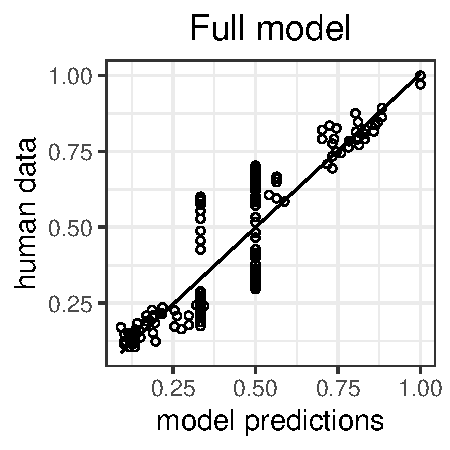
\includegraphics[width=2in]{images/m23.pdf}
	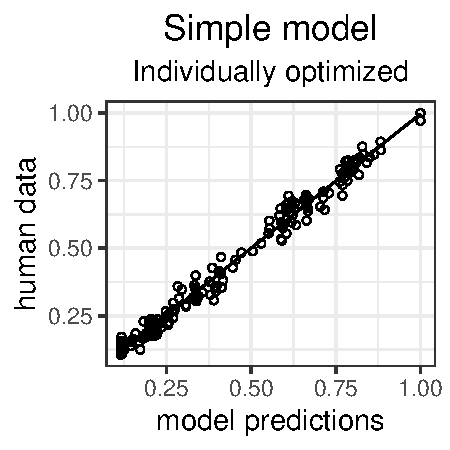
\includegraphics[width=2in]{images/m8.pdf}
		\caption{Human data from Experiment 1 plotted against the predictions of our simple model. % and fullPSIRSA
		Each data point indicates the slider values and model-predicted feature-preference posteriors for a particular ambiguity class.
		Left panel: $\gamma$ \emph{optimized globally} ($r^2 = 0.8614$); 
%		right panel: \emph{full model} ($r^2 = 0.8576$).}
		right panel: $\gamma$ and $\beta$ \emph{optimized individually} with leave-one-out cross-validation ($r^{2}=0.9901$).
	}
	%\label{cross-validation}
		\label{simple-global-and-cross-validated}
\end{figure}

%\gcs{how was the fitting performed?}

\subsubsection{Individually-fitted models}

We now compare our two model variants further when fitting the parameters to the individual data of each participant separately. In situations when the population is potentially heterogeneous, individual-level modeling in reference games improves the fit of the model despite its increased complexity \cite{franke2016reasoning}.
We optimized $\alpha$ and $\gamma$ in light of the KL divergence between the individual participants' slider-value choices and the corresponding model predictions.
We then again averaged the individualized model prediction values and participants' slider values with respect to the particular ambiguity classes and calculated correlations between the data and the model.


	\begin{table}[t]
		\centering
		\begin{tabular}{p{4.5cm}ccc}
			\hline
			Model & $r^2$ & $df$ & $F$  \\
			\hline
			
			\hspace{1cm}\textit{Simple model} & & &  \\
			
			Softness $\gamma$ & 0.8631 & 1,190 & 1205  \\
			Softness $\gamma$ \& Obedience $\beta$ & 0.9919 & 1,190 & 23480  \\
			
			\hspace{1cm}\textit{Full model} & & & \\
			
			Softness $\gamma$ \& Utility $\alpha$& 0.8627 & 1,190 & 1201 \\
			\hline
		\end{tabular}
		\caption{Optimization summary (individual) for Experiment 1 model predictions.}
		\label{individual}
	\end{table}



%Figure~\ref{simple-full-individual} shows that 
As Table \ref{individual} shows, the full model optimized at the individual level for the additional parameter $\alpha$ does not improve the fit compared to the simple model when both models are optimized for $\gamma$ (simple: $r^{2}=0.86$; full: $r^{2}=0.86$). 
Seeing that both models again fit the data nearly equally well (if anything, the simple model performs slightly better), we only consider the predictions of our simple model henceforth.
%
%
%%the For example, if a $S_2$ observes that following an utterance $blue$ and three objects all three of which are blue, but all differ in shape, the speaker chooses a square, the speaker might conclude that the $L_1$  has a preference for squares. However, the exact value on the slider the $S_2$ picks depends on the $\gamma$ parameter: if it is close to $0$, the speaker will mark that the $L_1$ had a perefernce for squares close to $1$. As the parameter value increases, the softness of preference will increase as well, drawing the preference value towards uniform (uninformative).
%%he model contains three parameters: the informativity paramter $\alpha$ (how informative speakers choose to be), the obey-instructions parameter $\beta$, and the softness of preferences parameter $\gamma$. The latter 
%
%% \gcs{We need to say something about how we fit individual participant data. How exactly where the parameter values fit? What were candidate values?}
%
%%\begin{figure}[ht]
%%	\centering
%%	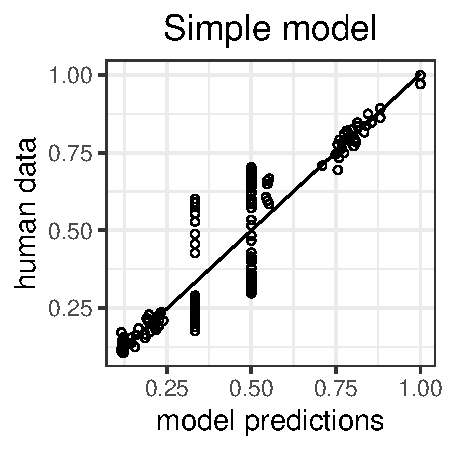
\includegraphics[width=2in]{images/m3.pdf}
%%	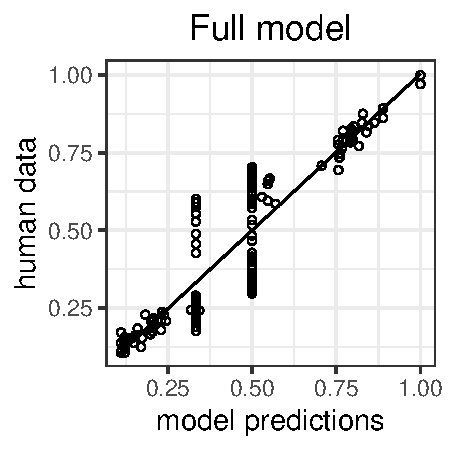
\includegraphics[width=2in]{images/m16.pdf}
%%	\caption{Human data from Experiment 1 plotted against the predictions of the \emph{individually} $\gamma$-optimized simplePSIRSA and the \emph{individually} $\gamma$- and $\alpha$-optimized fullPSIRSA models.}\label{simple-full-individual}
%% \end{figure}
%
%
%
%%When compared to the uniform-distribution base model, optimizing $\gamma$ alone yielded a much lower KL divergence value: while the uniform base model yields an average KL divergence of $9.848$ (median=$7.028$), our extended RSA model with individually-optimized $\gamma$ parameters yielded an average KL divergence of $2.058$ (median=$1.524$). 
%%When optimizing $\alpha$ and $\gamma$ together, a yet smaller average KL divergence of $1.451$ (median=$0.952$) is reached.
%%In the light of the $G^2$ statistics and under the assumption that we calculated $2$ KL divergences in all $15$ trials per participant, the KL values should be multiplied by $2*15*2=60$ to yield a $G^2$ estimate, although one may want to consider the two KL divergences in each trial as closely related, such that $2*15=30$ may be considered as a more passive multiplier.
%
%
%%With this factor, we get a difference of $233.7$ between the uniform base model and the one-parameter extended RSA model, while the additional optimization of $\alpha$ improves $G^2$ further by a value of $18.21$. Both of these results are far above the cutoff value of $6.63$ for $p=.01$, assuming a Chi-square distribution \cite{Lewandowsky:2011}. 
%%Thus, the extended model exceeds the uniform base model with very high likelihood. 
%%However, considering the much smaller improvement due to the additional optimization of $\alpha$, we analyze correlations with respect to the one-parameter (i.e., $\gamma$-optimized) model in what follows. 
%
%%When considering the distribution of optimized parameters, we can identify three participants who cause the optimization process to yield $\gamma$ values above $100$, indicating lazy participants who simply leave the slider values unadjusted. 
%%Another 15 participants yielded a $\gamma$ value above $1$, which indicates that they are considering preferences only to a small extent. The rest (i.e., 64 participants) yielded values below $1$, indicating a strong consideration of preference inferences in line with the model. 
% 
%%We compared  in the light of the distinguishable interpretation cases. 
%
The model fit of the simple model improves considerably when we additionally fit the obedience parameter $\beta$ at the individual level ($r^2=0.99$). 
%We plot predictions from the $\beta$- and $\gamma$-optimized model in Figure~\ref{cross-validation}, 
%Here the model explains a large proportion of variance in the human judgments ($r^2 = 0.9919, F(1,190) = 23480$). 
The likelihood ratio test (two-tailed) revealed that a $\gamma$- and $\beta$-optimized simple model provides a better fit compared to a model optimized only for $\gamma$ ($G^2 = 237.36, \textrm{df} = 82, p < 0.01$). The more complex model contains one additional parameter $\beta$ fitted for each subject, giving us 82 degrees of freedom. We additionally checked the generalizability of the model by performing leave-one-out cross-validation on the individual level. Figure~\ref{simple-global-and-cross-validated} shows that the resulting cross-validated model predictions retain the strong fit ($r^2 = 0.99, F(1,190) = 18910$).

%\begin{figure}[ht]%
%	\centering
%	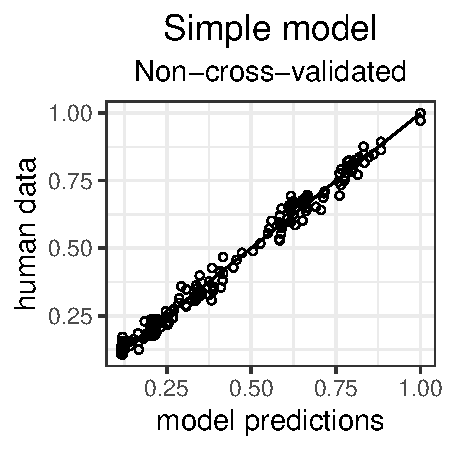
\includegraphics[width=2in]{images/m5.pdf}
%	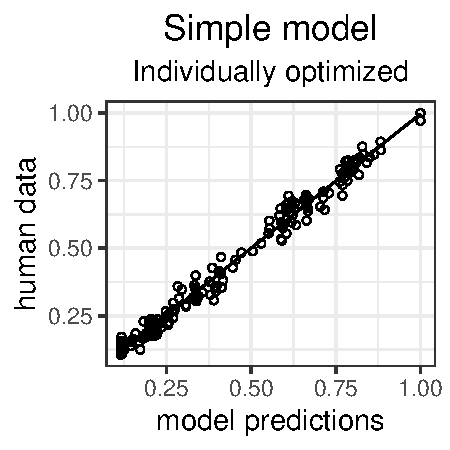
\includegraphics[width=2in]{images/m8.pdf}
%	\caption{Human data from Experiment 1 plotted against the predictions of the \emph{individually} $\beta$- and $\gamma$-optimized simplePSIRSA model. Left panel: \emph{non-cross-validated} ($r^{2}=0.992$); right panel: \emph{cross-validated} ($r^{2}=0.9901$).}\label{cross-validation}
%\end{figure}

It bears noting that the individually-fitted parameters do not improve the correlation values much, if at all, when compared to the globally-fitted model.  To appreciate the gains obtained by fitting model parameters, Figure~\ref{barplot_x4} shows the average responses of the human participants and of the individually-, two-parameter-optimized simple model and the non-optimized simple model for the scene type of the sample trial from Figure~\ref{exp1-trial}.
In that trial, participants saw that the middle object was chosen following the utterance ``red". There are two potential referents for this description: the red striped cloud and the red dotted circle. Since the cloud was chosen, we infer that the person who chose this object has a preference for clouds over circles, and for striped objects over dotted ones. 
Note that we cannot learn anything about the preference for solid things or squares in this trial because these features are not present, thus we ignore the respective slider values. 
Moreover, we can definitely not learn anything about color preferences because the color was uttered; thus, sliders for those features were not present.  
As Figure~\ref{barplot_x4} shows, both humans and the models assign high slider values to clouds and striped things, and low values to circles and dotted things. Indeed, even the non-optimized model fits the qualitative pattern of the results; optimizing $\beta$ and $\gamma$ improves the quantitative fit.


\begin{figure}[ht!]
	\centering
	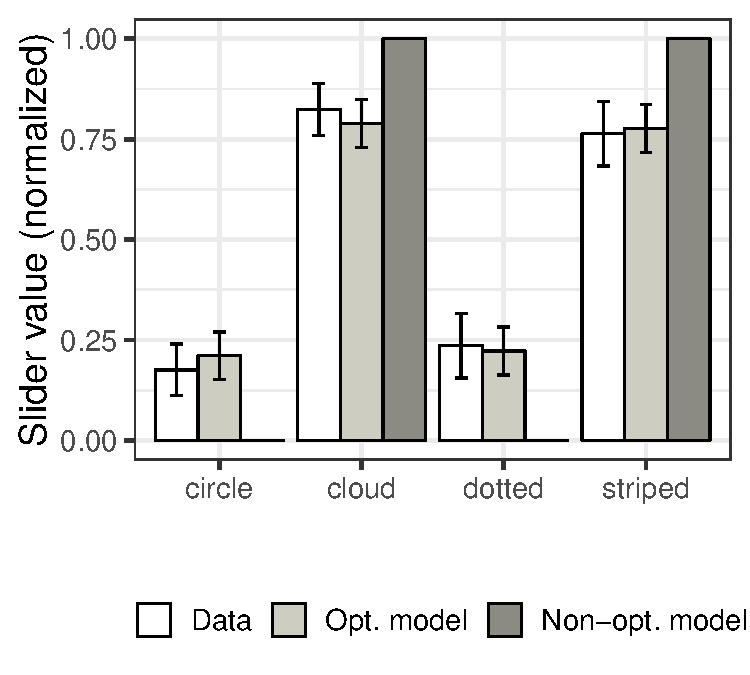
\includegraphics[width=2.5in]{images/december_barplot_x4.pdf}
	\caption{Human data and predictions from the simple model (individually-, two-parameter-optimized and non-opimized) for the scenario $S$ shown in Figure~\ref{exp1-trial}. Error bars represent 95\% confidence intervals.}\label{barplot_x4}
\end{figure}


We thus find strong empirical support for our simple model, implying that speakers are indeed able to use listener behavior to acquire information about their preferences. We fail to find that the full model predicts the data better.
This result suggests that the task in our experiments does not require full-blown pragmatic inference about alternative utterances.
% Martin: let's leave this statement out - it may annoy reviewers: 
% , in contrast with \citeA{frankgoodman2012} but in line with \citeA{sikos2019}. 
%There speakers needed to signal a particular object to the listener, while in our experiments the intention of the speaker is quite different: she produces an utterance to create a situation of ambiguity resolution. In turn, it is not the listener's goal to infer what object was intended as a referent; rather the listener picks an object according to her preferences.
The question now turns to whether speakers are able to capitalize on this reasoning when it comes to selecting utterances. In other words, are speakers aware that ambiguous language is potentially more informative and thus can use ambiguous language in a socially epistemic, strategic manner?

\section{Experiment 2: Choosing utterances to learn \\ about others} \label{experiment2}

Our next task is to check the predictions of our strategic utterance-selection model: given a set of potential referents $S$, are participants able to reason pragmatically about the anticipated potential epistemic utility of utterances $u\in U$ for inferring the listener's preferences? 
%


\subsection{Participants}

We recruited $90$ participants with US IP addresses through Amazon.com's Mechanical Turk crowdsourcing service; participants in Experiment 1 were not eligible to participate in Experiment 2. Participants were compensated for their participation. On the basis of a post-test demographics questionnaire, we again identified 82 participants as native speakers of English; their data were included in the analyses. We obtained a confirmation from all participants that they agree to participate in the study.

\subsection{Design and methods}

Participants encountered a reference game scenario similar to Experiment 1 in which a speaker signals an object to a listener who might have a preference for certain types of objects. However, rather than observing the utterance and referent choice, participants were now tasked with helping the speaker choose an utterance that was ``most likely to reveal the listener's color, shape, or pattern preferences.'' Figure \ref{exp2-trial} shows a sample trial, in which the speaker (``Katie'' in the example) is to choose an utterance in order to learn about the listener's preferences (``Elizabeth'' in the example). While the ambiguous utterances ``cloud'', ``green'', and ``striped'' may allow inferences about color \& texture, shape \& texture, and color \& shape, respectively, the utterances ``solid'', ``blue'', and ``circle'' leave only one response option to the listener, such that the speaker cannot learn about the listener's preferences when observing the listener's response (assuming the listener obeys the speaker's order).  


\begin{figure*}[ht]
	\centering
	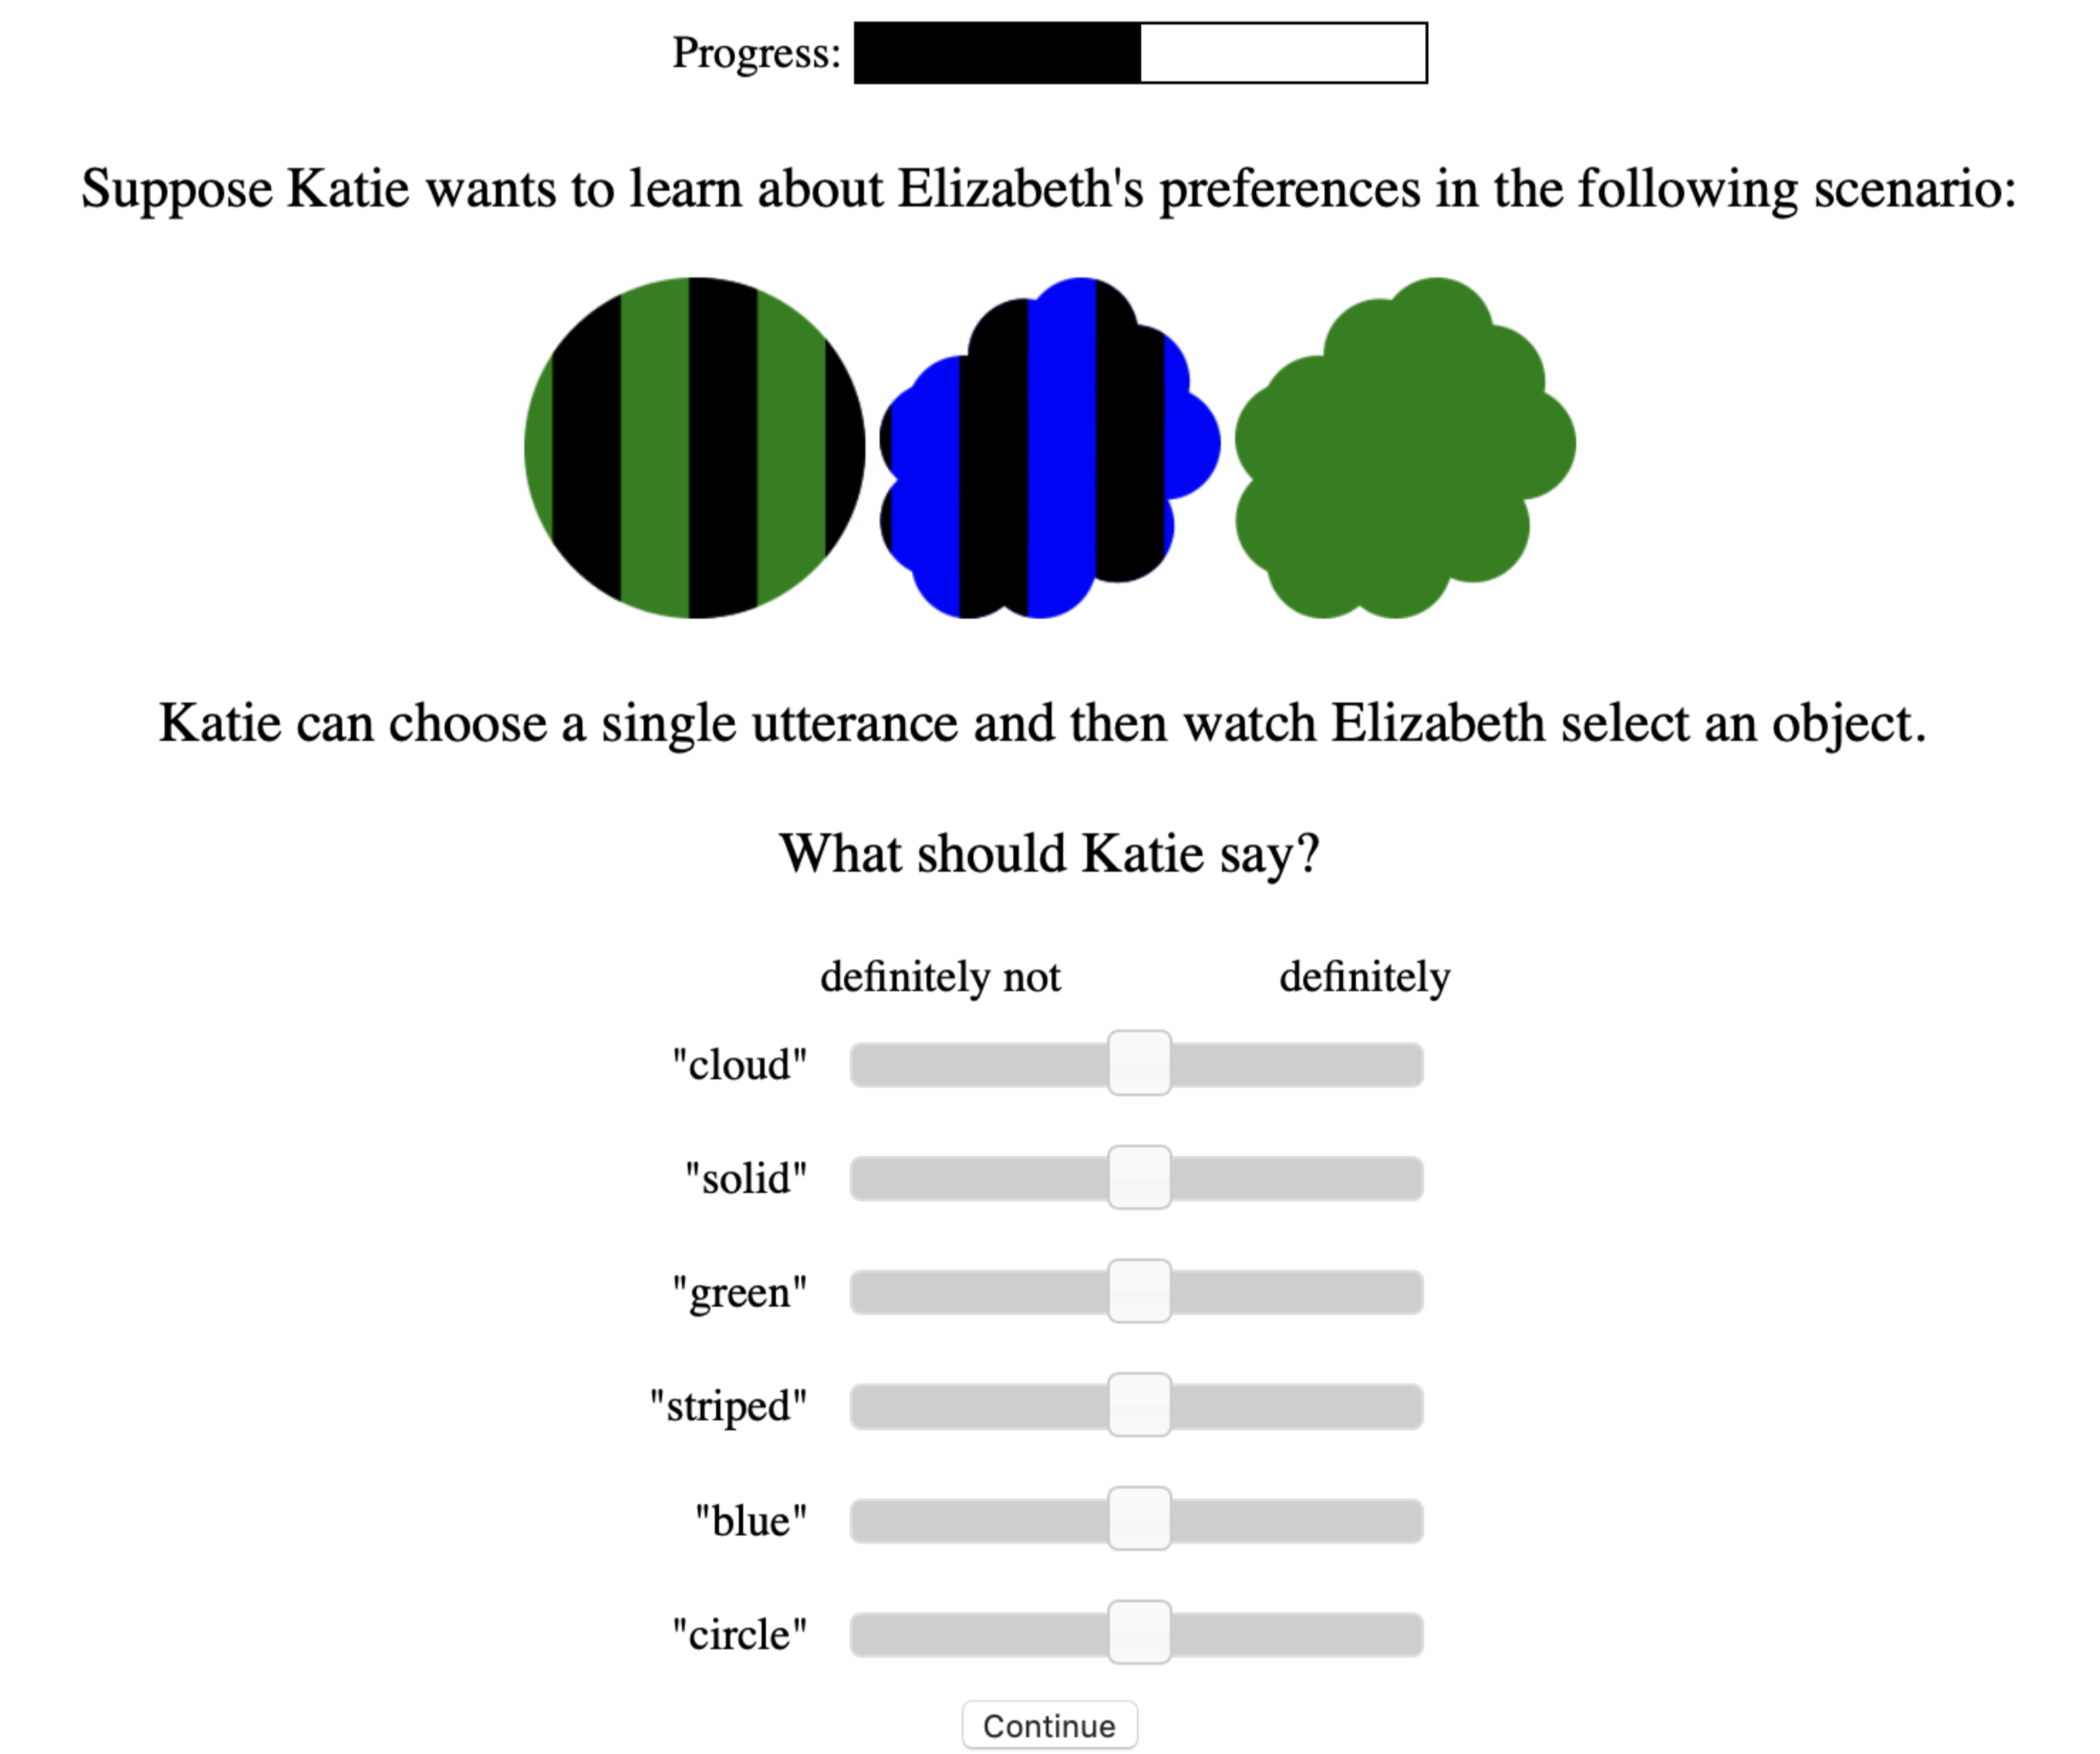
\includegraphics[width=4.5in]{images/utterance-choice-trial.png}
	\caption{A sample trial from \emph{Experiment 2: Choosing utterances}. }\label{exp2-trial}
\end{figure*} 


We used the same sets of objects from Experiment 1, which could vary along three dimensions. Each trial featured a set of three objects, as in Figure \ref{exp2-trial}. After observing the objects, participants adjusted sliders to indicate which single-feature utterance the speaker should choose to learn about the preferences of their listener. Potential utterances corresponded to the features of the objects present; depending on the number of unique features, participants adjusted between three and nine sliders. As with Experiment 1, we averaged the data and the respective model predictions across specific ambiguity classes, which include all scenes that yield identical utterance choice options. 
In this case, $14$ distinct conditions can be identified, with a total of $84$ slider values to set. 
Membership within an ambiguity class is defined by how many objects in a scene share each of the features: shape, pattern, and color. If objects share a feature, we also consider whether these objects also share other features. For example, in Figure \ref{exp2-trial}, two green objects differ in shape, making the utterance \textit{green} informative. If, on the other hand, both green objects were clouds, uttering \textit{green} would not allow the speaker to update their beliefs about the listener's shape preferences.
In the most extreme case, when all objects share all three features, all utterances are ambiguous since multiple objects can always be picked; but no utterance allows the speaker to learn anything about the listener because the object choice is uninformative. Another extreme case is a situation where all objects are unique and do not share any features. In such a case, any utterance will only pick one object, making learning about preferences impossible unless obedience ($\beta$) is not 0---that is, unless listeners have a tendency to disobey the utterance and consider objects that do not satisfy its literal interpretation.

Just like for Experiment 1, each ambiguity class yields unique model predictions for the individual features present in the respective scenarios $S$, taking into account their ambiguity role. This grouping strategy effectively distinguishes all model-relevant cases. Please see the Appendix for examples of different classes.


Participants completed a series of fifteen trials. As with Experiment 1, objects were chosen at random, with the constraint that ten trials were potentially informative with respect to the listener's preferences (as in Figure~\ref{exp2-trial}) and five trials were uninformative with respect to the listener's preferences (e.g., observing a set of three identical objects).

\subsection{Results}

%To reason about the utterance choosing strategies of $S_1\textrm{-simp}$, 
We use our simple model to compute the expected most-informative utterance for inferring preferences.
In other words, $P_{S_1\textrm{-simp}}(u)$ calculates the probability that a speaker would choose $u$ for the purpose of inferring preferences.

To generate predictions from $P_{S_1\textrm{-simp}}(u)$, three free parameters can be identified:
the preference softness $\gamma$, the obedience $\beta$, and the $\lambda$ parameter, which factors the importance of choosing the expected most-informative utterance with respect to the expected KL divergence between preference priors and expected preference posteriors 
(cf.~equation \ref{eq:kldivlambdasimp}). 
%It scales the expected information gain. 
While a positive $\lambda$ value yields the intention to maximize information gain, 
a negative value results in a tendency to minimize information gain, that is, a preference for no change in the posterior feature preference estimate $P_{S_{1\textrm{-simp}}}(f\mid u,s)$, in comparison to the prior estimate $P(f)$. 
A value of $\lambda=0$ effectively ignores information gain and a resulting tendency to choose the object that was most likely referenced given the $utterance$.
% Martin - this information can be found at the end of the methods section
%Note that negative values for $\lambda$ results in a minimization of expected information gain, effectively favoring unambiguous utterances. 
%Moreover, when $\lambda=0$, the model collapses to an approximate uniform distribution over the available utterances.
%\gcs{is this true? Will utterances that can describe more objects be preferred?}. Asya: verified with Martin, the description is correct.


%The proper model fit is confirmed when considering the correlation between the participants' data and the model predictions. 

We compare the performance of our simple model with the performance of a uniform baseline model, which merely chooses one of the available utterances at random. 
Seeing that in particular ambiguity cases with particular constellations $S$ up to nine utterances are possible, the baseline model yields different model predictions for the available utterances in the respective ambiguity classes. 
As a result, the baseline model is much better in capturing variance in the data than one would expect without this insight ($r^2 = 0.75$; Table \ref{utterance_optimization}). The non-optimized simple model, surprisingly, captures very little variance in the human data ($r^2=0.06$); for  the non-optimized model we set the parameters to hard preference and full obedience ($\gamma=0$, $\beta=0$) and the information gain factor $\lambda$ to $1$, thus preferring to choose those utterances that are expected to yield high information gain. Figure~\ref{base-nonopt-x3} compares the performance of this non-optimized simple RSA model with the baseline model that relies on a simple heuristic of distributing the probability mass equally among all utterances that are available in a scene.
%($r^2=0.7466$, $F(1,82) = 245.6$, $p<0.001$).

	\begin{table}[htb]
	\centering
	\begin{tabular}{p{3.2cm}cccccc}
		\hline
		Model & $r^2$ & $df$ & $F$ & Soft. $\gamma$ & Obed. $\beta$ & Inf. gain $\lambda$ \\
		\hline
		
		Baseline & 0.7466 & 1,82 & 245.6 && & \\
		Non-optimized & 0.0595 & 1,82 & 6.253 &&& \\
		
		Softness \& Obedience \& Inf. gain & 0.7991 & 1,82 & 331.2 & 0.0006 & 0.2758 & 0.3663 \\
		\hline
	\end{tabular}
	\caption{Experiment 2. Optimization summary (global).}
	\label{utterance_optimization}
\end{table}

\begin{figure}[ht]
	\centering
	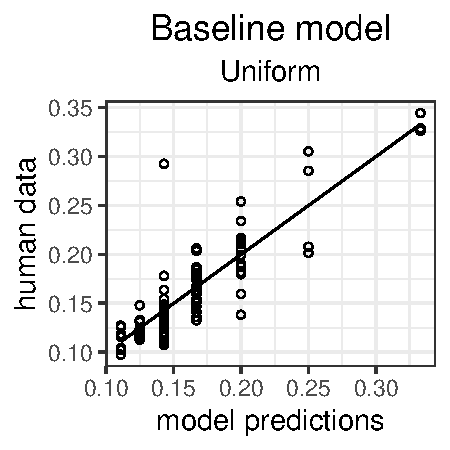
\includegraphics[width=2in]{images/x3_m20.pdf}
	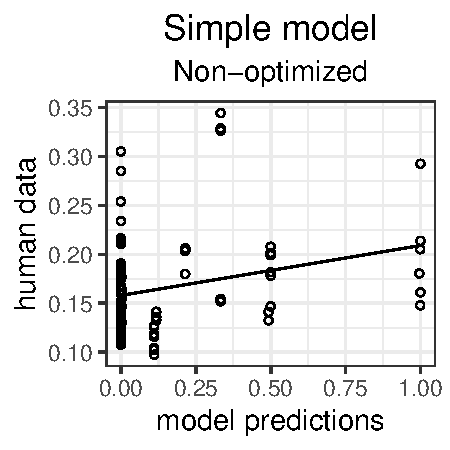
\includegraphics[width=2in]{images/x3_m7.pdf}
	\caption{Average human data from Experiment 2 plotted against the predictions of the uniform baseline model (left; $r^2=0.75$) and the simple model (right; $r^2=0.06$). 
%		Left panel: \emph{uniform model} ($r^{2}=0.7466$);
%		right panel: \emph{non-optimized simple model} ($r^2=0.0595$).
	}
	\label{base-nonopt-x3}
\end{figure}



To examine the reasons for this failure of the non-optimized simple model, we first performed additional global parameter optimization runs.
As Table \ref{utterance_optimization} shows, when optimizing all of the simple RSA model parameters, the model accounts for more variance than the uniform base model 
%($r^2=0.7991$, $F(1,82) = 331.2$, $p<0.001$; optimized model parameters: $\gamma=0.0006$, $\beta=0.2758$, $\lambda=0.3663$).
%A nested-model-comparison test with three free parameters yields a 
($r^2=0.80$; $G^2 = 13.6912,  p<0.01$); Figure~\ref{global-individual-x3} (left) shows the correlation plot. 
The estimated parameter values ($\gamma=0.0006$, $\beta=0.2758$, $\lambda=0.3663$) indicate that the preference strength is rather high, obedience is not as strong, while the information gain intention is present but moderate.
%(Table \ref{utterance_optimization}). 
%We now turn to individual parameter optimization, suspecting that their may be fundamental differences between the individual participants. 



%Figure \ref{exp2-results} plots predictions from the $\lambda$-optimized model, together with the human data. Again, we observe a strong positive correlation between the human judgments and model predictions ($r^2 = 0.91, p < 0.001$). In other words, we find evidence in support of the idea that speakers reason pragmatically about the relative informativity of ambiguous language.


% I recorded the same number of conditions as in Experiment 1. I think Experiment 2 used the same ambiguity code.

%The results for the base model yielded an average KL divergence value of $5.415$ (median=$3.997$), while the $\lambda$-optimized model yielded a mean KL divergence of $3.774$ (median=$2.108$).
%Again determining $G^2$ to enable a Chi-square test for significant model differences in fitting the data, the difference between the base model and one-parameter model (factored by $2*15=30$) of $49.23$ (median difference of $56.67$) is highly significant, indicating that the one-parameter model fits the data much better than a uniform base model. 
% Note: these interesting observations may not be mentioned _ I leave them in for now because the discussion can relate to them 


Turning to individual parameter optimization, we compared three single-parameter-individually-optimized simple RSA models to determine which model provides the best fit to the data. 
All models have similar levels of complexity, with either softness $\gamma$, obedience $\beta$, or the KL-factor $\lambda$ being optimized.
The results indicate that we get the best fit by optimizing the KL-factor $\lambda$ ($r^{2}=0.9059$, $F(1,82) = 800.2$; leave-one-out cross-validated optimization $r^{2}=0.8902$, $F(1,82) = 664.8$), with other models capturing less variance in the data ($\beta$-optimized $r^{2}=0.8015$, $F(1,82) = 336.1$; $\gamma$-optimized $r^{2}=0.8077$, $F(1,82) = 349.6$).
The comparison with the baseline model in terms of nested model statistics confirms that only the individual optimization of $\lambda$ improves model performance ($\lambda$: $G^2=268.88$, $\textrm{df}=82$, $p<0.001$; $\gamma$: $G^2=31.38$, n.s.; $\beta$: $G^2=56.29$, n.s.).
Two- and three-parameter individual optimizations did not yield any significant model improvements when compared to the individually-$\lambda$-optimized model (best improvement when optimizing $\gamma$ in addition to $\lambda$: $G^2=24.72$, $\textrm{df}=82$, n.s.).
% were unstable due to parameter interactions; therefore, we do not report the results for those models.
Figure~\ref{global-individual-x3} (right) shows the resulting correlation plot for the individually-$\lambda$-optimized model. 
 
\begin{figure}[ht]
	\centering
	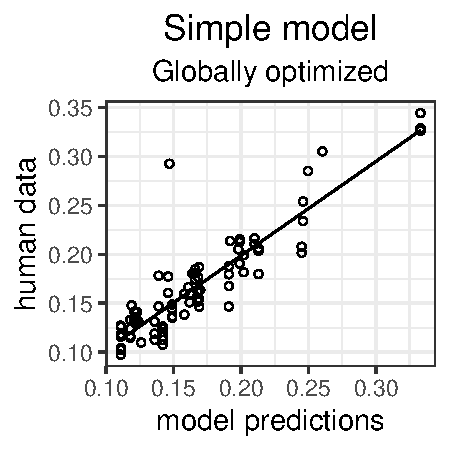
\includegraphics[width=2in]{images/x3_m24.pdf}
	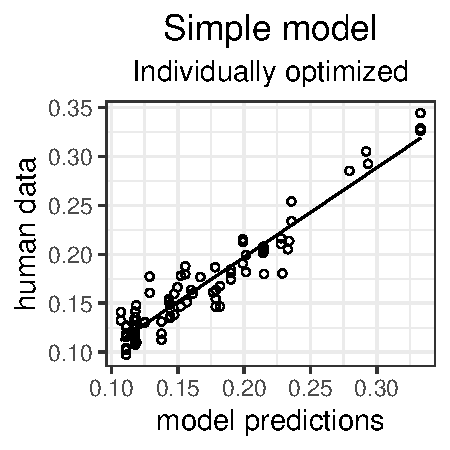
\includegraphics[width=2in]{images/x3_m11.pdf}
	\caption{Average human data from Experiment 2 plotted against the predictions of the optimized simple models.
		Left panel: \emph{globally-optimized three-parameter model} ($r^{2}=0.7466$;
		right panel: \emph{individually-$\lambda$-optimized model} ($r^{2}=0.9059$). }
	\label{global-individual-x3}
\end{figure}


Unlike for Experiment 1, where even the non-optimized models provided a good linear fit to the data, optimization produces a large effect on the model predictions in Experiment 2.
Figure~\ref{barplot_x3} compares individually-optimized vs.~non-optimized model predictions against the human behavior for the sample trial in Figure~\ref{exp2-trial} \gcs{would it be easy to show also the globally-optimized predictions in this plot?}.
We see that the non-optimized model strongly favors ambiguous utterances: in a situation with a green striped circle, a blue striped cloud, and a green solid cloud, uttering things like \textit{cloud}, \textit{striped}, or \textit{green} (i.e., the utterances that point to more than one object in the scene) could let the speaker learn something about the listener's preferences.
However, Figure~\ref{barplot_x3} shows that human behavior deviates quite strongly from the non-optimized, ambiguity-selecting baseline; once we optimize $\lambda$, we are able to capture human behavior in the task.
%For example, \textit{green} picks out two objects: a striped green circle and a solid green cloud; after saying ``green'', the speaker could learn whether the listener prefers striped things over solid things, or circles over clouds.

\begin{figure}[ht]
	\centering
	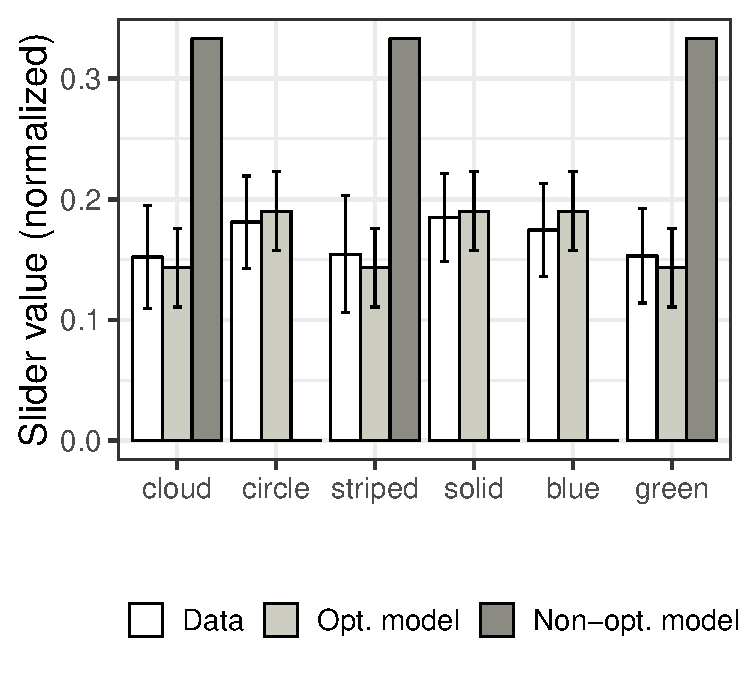
\includegraphics[width=2.5in]{images/december_barplot_x3.pdf}
	\caption{Model predictions and human data for the ambiguity class in in Figure~\ref{exp2-trial}.
	 %one of the classes of stimuli \emph{Experiment 2: Picking utterances}. 
	 The optimized version of the model is optimized for the KL-factor $\lambda$. Error bars represent 95\% confidence intervals.}\label{barplot_x3}
\end{figure}

% Note: I did check it - there are indeed 14. 5+5+6+7+6+6+7+3+4+5+6+7+8+9
%After matching the respective actual feature values with the utterance choice relevant within the respectively-binned conditions, we again computed averages over utterance preference values for the respectively-binned trials across participants and across respective model predictions \gcs{this is awfully hard to follow}. Asya: decided to remove this part, reordering can just as well stay behind the scenes.

% Asya: Need to fix the text below 
%In Figure~\ref{kl-factor}, 
%In Figure \ref{kl-factor}, we compare $\lambda$-optimized simplePSIRSA (right panel) with a uniform base model (left panel), which assigns equal probability to each utterance available for a particular context.
%This baseline model essentially has no utterance  preferences whatsoever, but reflects the fact that the ambiguity classes distinguish between cases with a different number of utterance choice options (i.e., three to nine).
 %\gcs{why is this a reasonable model to compare against? I think we need to do more to motivate this comparison.}. 
 %\gcs{how is this model defined?} Asya: it really is a model that takes the probability of 1 and distributes it evenly between all possible utterances.
 %Since simplePSIRSA with $\lambda=0$ collapses to the baseline model, optimizing the $\lambda$ %parameter in simplePSIRSA is a nested model. 
 %When statistically comparing the individually-optimized $\lambda$ simplePSIRSA model with the baseline model, the likelihood ratio test confirms that individual $\lambda$ optimizations yield better fits than the baseline model ($G^2 = 268.87, \textrm{df} = 82, p <0.01$).

When examining the individually-optimized model values in further detail, we noticed three groups of participants. 
The first one may be termed a ``lazy worker'' or ``unpredictable behavior'' group:
for $28$ participants, the KL divergence values of the $\lambda$-optimized simple RSA model failed to reach the performance of the baseline model, essentially failing to identify any model-corresponding regularity in the data that goes beyond random utterance choice behavior.
%The first one is a ``lazy worker'' group of $18$ participants whose fitted $\lambda$ values were close to zero (i.e.,  $-.02 < \lambda<.02$), indicating that they were randomly selecting utterances.
The second group of $33$ participants yielded more negative values (i.e., $-7.11<\lambda<-0.014$, $\bar{\lambda}=-0.823$), indicating that a significant number of participants preferred to systematically choose unambiguous utterances ($G^2=180,17$, $\textrm{df}=33$, $p<0.001$). 
The third group of $21$ participants yielded positive values (i.e., $.0187<\lambda<.537$, $\bar{\lambda}=-0.124$), indicating that these participants indeed preferred the more ambiguous utterances in a strategic manner ($G^2=102.16$, $\textrm{df}=21$, $p<0.001$).


Further experiments with highly similar setups confirmed this trend.
In particular, we ran two additional, complementary studies with a blocked design where participants first completed preference-inference trials as in Experiment~1 and then utterance-selection trials as in Experiment~2. 
In the first complementary study with 10 trials (135 participants, data from 123 native speakers of English included in the analysis, 12 non-native speakers excluded), an identical analysis yielded $42\%$ of participants that preferred ambiguous over unambiguous utterances ($37\%$ unpredictable participants; $21\%$ preferred unambiguous utterances). 
In the second complementary study with 54 participants (two participants excluded as non-native speakers), which contained 30 trials in total and had slightly more general instructions, as many as $64\%$ of the participants systematically preferred ambiguous over unambiguous utterances ($21\%$ unpredictable workers; $15\%$ preferred unambiguous utterances). 



\section{Discussion} \label{discussion}

The ability to infer the intentions and goals of others upon observing their behavior develops early in ontogeny and remains a valuable source of information for building predictive models of others. 
%Previous work in the RSA framework has focused on jointly inferring the meaning of utterances and the state of the world based on the speaker's choice of utterances \cite{degen2015wonky, hawkins2015you} and the iterative vocabulary learning tasks that involve the inference about the priors of the speaker  \cite{woensdregt2016modelling, blokpoel2019pragmatic} \gcs{are these RSA models? I don't think so..}.
In this paper, we asked whether communicative behavior---specifically the resolution of ambiguous reference---provides interpretable data for speakers to learn more about their listeners.

We have found strong support for the idea that speakers can indeed learn about others when observing their interpretation of ambiguous utterances. This result connects our findings to the Bayesian Theory of Mind literature that describes how children and adults use observable behavior to infer the mental states of others.
% for PSIRSA, which infers preference posteriors on the basis of ambiguous language.
% \gcs{we might want to talk about this as ``priors'' in the introduction as well} Asya: added a new section to the Intro
The results of Experiment~1 demonstrate that na\"ive speakers are able to reason pragmatically about \emph{why} listeners may take the actions they do in cases of referential ambiguity. 
The success of our computational model in predicting the observed behavior offers an articulated hypothesis about \emph{how} this reasoning proceeds: when speakers are aware of the ambiguity in their utterances, observing how listeners resolve that ambiguity provides clues about the preferences listeners use when doing so.
The results of Experiment 2 demonstrate that at least some speakers are able to capitalize on this reasoning to strategically select ambiguous utterances that are expected to improve their understanding of the preferences of their listeners.

% \gcs{our simple model doesn't actually have a listener reasoning about a speaker}
%By modeling the inference process within the RSA framework, we conceptualize the utterance interpretation process as the recursive reasoning of speakers and listeners about each other. We thereby bring together the rich literature on Bayesian models of inferences (e.g., naive utility calculus) on the one hand and the modeling of pragmatic reasoning on the other. Both of these approaches are based on the view of the agent/speaker as a utility-driven agent, and it is the reasoning about the speaker's optimal behavior that drivers the listener's interpretation of the utterance.  We focused on modeling the speaker behavior that spans beyond efficient information transfer, and rather is aimed at generating interpretative options that could be informative as possible choices.

One might question the ecological validity of this epistemically-motivated ambiguity behavior. Intuitively, such a strategy appears to be a sub-optimal way to elicit information when compared to a direct question---in the case of our experiments, a question about the preferences of the listener. Yet, considerations of politeness \cite{yoon2018polite} or a general rhetorical strategy of indirectness could make the costs of asking a question prohibitively high. For example, asking a stranger directly about her political views might appear impolite or even aggressive, while making a vague statement about the course of an election by stating that their results are `interesting' could act as a probe to get the opinion of the listener without forcing her to react. Evidence from a corpus of speed-dating dialogues suggests that direct questions in situations of courtship---supposedly a setup that should promote information-seeking behavior---are a sign that the interaction between the partners is not going as smoothly as possible \cite{mcfarland2013making}; to facilitate a stalled conversation, speakers have to ask a question rather than continue the flow of the previous discussion.

The results of our utterance-choice experiment (Experiment 2) suggest that not all speakers can strategically select ambiguous utterances to yield situations of ambiguity resolution. Two explanations may be warranted and need to be investigated further. 
First, it may be the case that these participants think overly egocentrically, thus having the intention to signal their own preferences rather than to give options to the listener. 
Second, it may simply be the case that these participants do not have access to the required deeper reasoning process, and thus prefer to give instructions with predictable outcomes. 
% \gcs{it might be good to speculate as to why only some of our participants selected ambiguous utterances: misunderstanding instructions, inability to follow instructions, or perhaps some other factor}
In fact, this special skill might only be present in speakers with high meta-linguistic competence, such as, for example, professional writers. They strategically use ambiguity to create an artistic effect of uncertainty about the interpretation of characters and events \cite{bade2015ambiguity, bauer2014dickens, quigley2015modernist}.


However, ambiguity does not need to be an explicit strategy of the speaker to make the inference process possible. Rather, ambiguity is naturally present in language as a consequence of economy considerations and indirectness strategies, providing ample interpretative freedom to the listener. In that sense, observing ambiguity resolution is a consequence not of active but rather retrospective inference that emerges once the speaker realizes that an utterance is potentially ambiguous. Taken together, the results of our experiments and modeling indicate that humans are aware of the fact that by observing responses to ambiguous utterances, information about the listener's prior preferences can be inferred---that is, they are able to learn about the hidden model states of others, including preferences but probably also other aspects of beliefs. 

% Currently, we are transferring the experimental setup to more naturalistic interaction scenarios. 
% Even in these cases, though, it appears that we still find a split among participants such that there are those who consistently prefer to choose unambiguous utterances. 

 %Our model infers an informative distribution over preferences of the listener, rather than resorting to a uniform prior in case the listener decides the world is wonky \cite{degen2015wonky}. 
% In addition to generating model predictions, we compare the model predictions to behavioral data, continuing the tradition of the RSA framework and setting this paper in contrast to other work that relies soley \gcs{is this true? no behavioral work?} on simulations of the interaction between two artificial agents \cite{woensdregt2016modelling,blokpoel2019pragmatic}. \gcs{maybe bring this up in the conclusion?}
 % Asya: yes, these two are simulation papers, no behavioral data
% However, unlike \citeA{hawkins2015you}, the epistemic goals of the speaker concern not the state of the external world but rather the mind of the listener. 
 

% Asya: Rephrased the following paragraph above
%It should also be noted that ambiguous utterances used in this way are closely related to questions, which may ask directly about considered preferences.
%Ambiguous utterances provide a ready but more subtle, indirect alternative to asking directly. 
%In normal conversations, a speaker might favor the indirect route, given considerations of politeness and possibly also in an effort to keep the conversation open. 
%With ambiguous language, the conversation partner can choose to disambiguate the ambiguous utterance or, alternatively, choose to continue in a different direction or even change topic.


We note that the analyzed preference prior, viewed from a broader perspective, can be closely related to a part of the event-predictive mind of the listener and the speaker \cite{Butz:2016,Butz:2017}.  This paradigm emphasizes the role of predictions in determining the success of our behavior. In order to anticipate the changes in the environment, including the behavior of other human agents, the predictive mind continuously updates its models of others by incorporating novel behavioral evidence.
When interpreting an utterance---in our experimental setup, opening up a set of referent choices---the listener's mind infers the current choices and integrates them with her preference priors, implicitly anticipating possible choice consequences.
Moreover, the expected information gain term---computing the utterance choice of the speaker---can be equated with the computation of socially-motivated active inference \cite{Butz:2017a, Clark:2016, Friston:2015}.
This inference causes the model to strive for an anticipated epistemic value that quantifies the expected information gain about the preferences of the listener---that is, expecting a form of social information gain. 
%More generally, predictive states of mind about others do not only include considerations of preferences, but may also concern all imaginable knowledge, opinions, beliefs, and current trains of thought of the listener.
%Moreover, during a conversation, the involved ``social'' priors will dynamically develop depending on the internal predictive models and the generated utterances, actions, and responses of the speaker and listener. 
%The priors dynamically depend on the privileged grounds of the conversational partners, and also on the common ground in which the conversation unfolds.
%In that sense, ambiguous utterances and resolutions thereof are one device for projecting parts of each other's privileged grounds into the common ground. 
In that sense, ambiguity resolution opens possibilities for conversation partners to make inferences about each others prior beliefs that span beyond the contents of the current conversation.



%Moreover, there 
%in conversation the priors dynamically unfold according to beliefs and preferences about the world and speakers
%twin anecdote, politeness (why not ask directly?)
%is ambiguity a feature that evolved under pressure from these considerations (i.e., informing preferences), or did ambiguity predate these considerations and speakers merely figured out clever ways of capitalizing on it---a lemonade-out-of-lemons scenario?





\section*{Funding}

This project has been funded by the Deutsche Forschungsgemeinschaft (DFG, German Research Foundation)--Project number 198647426. 

\section*{Data availability}
Data supporting the findings of this study are available from the corresponding author upon request.

\bibliographystyle{apacite}
\setlength{\bibleftmargin}{.125in}
\setlength{\bibindent}{-\bibleftmargin}

\bibliography{prior-inference}

\cleardoublepage

\appendix

\section{Ambiguity classes}

\subsection*{Experiment 1}

Figure~\ref{fig:ambiguity-classes-exp1} shows three exemplar scenarios for three representative ambiguity classes. 
Let us consider the first class in more detail.
In the scenario $S$ on the left side of Figure~\ref{fig:ambiguity-classes-exp1a}, 
the utterance ``blue'' refers either to the blue square or the blue circle.
The picked object, that is, the blue circle, is unique in its shape (circle) and shares the other non-referenced property with both other objects (that is, its solid pattern). 
The referenced but not picked object (that is, the blue square), shares its shape with the non-referenced object. 
In the scenario $S$ in the center, the referenced two red objects differ in texture but share shape with the non-referenced object.
In the scenario $S$ on the right, the referenced two solid objects can be contrasted in their color but share their shape with the third object.



\begin{figure*}[htb]
	\centering
	\begin{subfigure}{\linewidth}
		\begin{subfigure}[b]{0.3\linewidth}
			\centering
			\begin{tikzpicture}
			\node[](o1) at (-1,0){
\includegraphics[width=.75cm]{appendix/311.png}};
			\node[](o2) at (0,0){
\includegraphics[width=.75cm]{appendix/211.png}};
			\node[](o3) at (1,0){
\includegraphics[width=.75cm]{appendix/313.png}};
			\draw[dashed, color=orange,line width=1mm] (o2.south west) rectangle ++(1.cm,1.cm);
			\node[] at ([yshift=10pt]o2.north){Utterance: \textbf{``blue"}};
			\end{tikzpicture}
		\end{subfigure}
		\hspace*{0.3cm}
		\begin{subfigure}[b]{0.3\linewidth}
			\begin{tikzpicture}
			\node[](o1) at (-1,0){
\includegraphics[width=.75cm]{appendix/212.png}};
			\node[](o2) at (0,0){
\includegraphics[width=.75cm]{appendix/213.png}};
			\node[](o3) at (1,0){
\includegraphics[width=.75cm]{appendix/222.png}};
			
			\draw[dashed, color=orange,line width=1mm] (o3.south west) rectangle ++(1.cm,1.cm);
			
			\node[] at ([yshift=10pt]o2.north){Utterance: \textbf{``red"}};
			\end{tikzpicture}
		\end{subfigure}
		\hspace*{0.3cm}
		\begin{subfigure}[b]{0.3\linewidth}
			\begin{tikzpicture}
			\node[](o1) at (-1,0){
\includegraphics[width=.75cm]{appendix/112.png}};
			\node[](o2) at (0,0){
\includegraphics[width=.75cm]{appendix/131.png}};
			\node[](o3) at (1,0){
\includegraphics[width=.75cm]{appendix/111.png}};
			\draw[dashed, color=orange,line width=1mm] (o1.south west) rectangle ++(1.cm,1.cm);
			\node[] at ([yshift=10pt]o2.north){Utterance: \textbf{``solid"}};
			\end{tikzpicture}
		\end{subfigure}
		\caption{The utterance potentially references two objects, the picked object has one non-referenced unique feature, while the other, non-referenced feature is shared among all three objects.
			The other referenced---but not chosen---object shares its other feature with the non-referenced object.} 
		\label{fig:ambiguity-classes-exp1a}
		%21 32 12
	\end{subfigure}
	%%%%%%     Subfigure Part 2
	%class 21 22 12
	\begin{subfigure}{\linewidth}
		\centering
		\begin{subfigure}[b]{0.3\linewidth}
			\centering
			\begin{tikzpicture}
			\node[](o1) at (-1,0){
\includegraphics[width=0.75cm]{appendix/133.png}};
			\node[](o2) at (0,0){
\includegraphics[width=0.75cm]{appendix/122.png}};
			\node[](o3) at (1,0){
\includegraphics[width=0.75cm]{appendix/232.png}};
			
			\draw[dashed, color=orange,line width=1mm] (o2.south west) rectangle ++(1.00cm,1.00cm);
			
			\node[] at ([yshift=10pt]o2.north){Utterance: \textbf{``red"}};
			\end{tikzpicture}
		\end{subfigure}
		\hspace*{0.3cm}
		\begin{subfigure}[b]{0.3\linewidth}
			\begin{tikzpicture}
			\node[](o1) at (-1,0){
\includegraphics[width=0.75cm]{appendix/133.png}};
			\node[](o2) at (0,0){
\includegraphics[width=0.75cm]{appendix/122.png}};
			\node[](o3) at (1,0){
\includegraphics[width=0.75cm]{appendix/232.png}};
			
			\draw[dashed, color=orange,line width=1mm] (o1.south west) rectangle ++(1.00cm,1.00cm);
			
			\node[] at ([yshift=10pt,xshift=0pt]o2.north){Utterance: \textbf{``polka-dotted"}};
			\end{tikzpicture}
			%		\subcaption{Another combination, here the polka-dotted objects differ in shape and color.}
		\end{subfigure}
		\hspace*{0.3cm}
		\begin{subfigure}[b]{0.3\linewidth}
			\begin{tikzpicture}
			\node[](o1) at (-1,0){
\includegraphics[width=0.75cm]{appendix/212.png}};
			\node[](o2) at (0,0){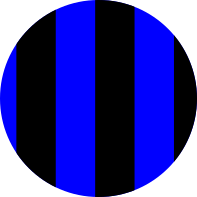
\includegraphics[width=0.75cm]{appendix/221.png}};
			\node[](o3) at (1,0){
\includegraphics[width=0.75cm]{appendix/311.png}};
			
			\draw[dashed, color=orange,line width=1mm] (o2.south west) rectangle ++(1.00cm,1.00cm);
			
			\node[] at ([yshift=10pt]o2.north){Utterance: \textbf{``circle"}};
			\end{tikzpicture}
			%	\subcaption{Two circles differ in texture and color.}
		\end{subfigure}
		%21 22 12
		\caption{The utterance $u$ references two objects whereby both objects only share the uttered feature. The third object shares one feature with each of the two referenced objects.}
	\end{subfigure}
	%%%%%%     Subfigure Part 3	
	\begin{subfigure}{\linewidth}
		\centering
		\begin{subfigure}[b]{0.3\linewidth}
			\centering
			\begin{tikzpicture}
			\node[](o1) at (-1,0){
\includegraphics[width=0.75cm]{appendix/131.png}};
			\node[](o2) at (0,0){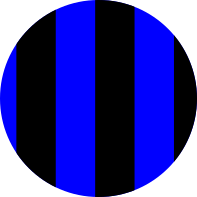
\includegraphics[width=0.75cm]{appendix/221.png}};
			\node[](o3) at (1,0){
\includegraphics[width=0.75cm]{appendix/231.png}};
			
			\draw[dashed, color=orange,line width=1mm] (o1.south west) rectangle ++(1.00cm,1.00cm);
			
			\node[] at ([yshift=10pt]o2.north){Utterance: \textbf{``blue"}};
			\end{tikzpicture}
			%		\subcaption{The objects can differ in shape, texture, and color. The utterance applies to all 3 objects but they differ in shape and texture. Solid objects or squares are absent here, so we cannot learn whether the listener likes squares or solid objects.}
		\end{subfigure}
		\hspace{0.3cm}
		\begin{subfigure}[b]{0.3\linewidth}
			\begin{tikzpicture}
			\node[](o1) at (-1,0){
\includegraphics[width=0.75cm]{appendix/123.png}};
			\node[](o2) at (0,0){
\includegraphics[width=0.75cm]{appendix/122.png}};
			\node[](o3) at (1,0){
\includegraphics[width=0.75cm]{appendix/112.png}};
			
			\draw[dashed, color=orange,line width=1mm] (o3.south west) rectangle ++(1.00cm,1.00cm);
			
			\node[] at ([yshift=10pt]o2.north){Utterance: \textbf{``cloud"}};
			\end{tikzpicture}
			%		\subcaption{Another combination, here all objects are clouds but the picked object shares being red with another object.}
		\end{subfigure}
		\hspace*{0.3cm}
		\begin{subfigure}[b]{0.3\linewidth}
			\begin{tikzpicture}
			\node[](o1) at (-1,0){
\includegraphics[width=0.75cm]{appendix/311.png}};
			\node[](o2) at (0,0){
\includegraphics[width=0.75cm]{appendix/211.png}};
			\node[](o3) at (1,0){
\includegraphics[width=0.75cm]{appendix/313.png}};
			
			\draw[dashed, color=orange,line width=1mm] (o2.south west) rectangle ++(1.00cm,1.00cm);
			
			\node[] at ([yshift=10pt]o2.north){Utterance: \textbf{"solid"}};
			\end{tikzpicture}
		\end{subfigure}
		\caption{In this third exemplar ambiguity class, the utterance refers to all three objects. The picked object shares one feature with one other object and has one feature just for itself while the other two objects share it.}
		%32 21 12
	\end{subfigure}
	\caption{Three exemplar scenarios $S$, constraining utterance $u$, and chosen object $s$ are shown for three exemplar ambiguity classes for Experiment 1.}
	\label{fig:ambiguity-classes-exp1}
\end{figure*}

\subsection*{Experiment 2}

Figure~\ref{fig:ambiguity-classes-exp2} shows three exemplar scenarios for three representative  ambiguity classes. 
Let us again consider the first class in more detail.
In the scenario $S$ on the left side of Figure~\ref{fig:ambiguity-classes-exp2a}, 
all three objects share the feature pattern (solid), while two share  color (blue), and the other two share shape (square).
As a result, uttering \textit{green} or \textit{circle} will unambiguously signal a single object to the listener because the utterance identifies one unique object. 
On the other hand, uttering \textit{solid} will let the listener choose freely, while uttering \textit{blue} or \textit{square} will give a specific choice between two objects, that is, between the blue circle and the blue square or between the blue square or the green square, respectively.
In the scenario $S$ in the center, the objects share shape (circle), two share pattern (solid), and the other two share color (red).
Here, \textit{circle} references all three objects, \textit{red} or \textit{solid} reference pairs of objects, and \textit{striped} or \textit{green} reference one unique object each.
In the scenario $S$ on the right, the objects again share shape (cloud), two share  pattern (solid), while the other two share color (blue).


\begin{figure*}[!htb]
	\centering
	\begin{subfigure}{\linewidth}
		\begin{subfigure}[t]{0.3\linewidth}
			\centering
			\begin{tikzpicture}
			\node[](o1) at (-1,0){
\includegraphics[width=0.75cm]{appendix/311.png}};
			\node[](o2) at (0,0){
\includegraphics[width=0.75cm]{appendix/211.png}};
			\node[](o3) at (1,0){
\includegraphics[width=0.75cm]{appendix/313.png}};
			
			\end{tikzpicture}
			%		\subcaption{}
		\end{subfigure}
		\hspace*{0.3cm}
		\begin{subfigure}[t]{0.3\linewidth}
			\begin{tikzpicture}
			\node[](o1) at (-1,0){
\includegraphics[width=0.75cm]{appendix/212.png}};
			\node[](o2) at (0,0){
\includegraphics[width=0.75cm]{appendix/213.png}};
			\node[](o3) at (1,0){
\includegraphics[width=0.75cm]{appendix/222.png}};
			
			\end{tikzpicture}
			%		\subcaption{Another combination, h}
		\end{subfigure}
		\hspace*{0.3cm}
		\begin{subfigure}[t]{0.3\linewidth}
			\begin{tikzpicture}
			\node[](o1) at (-1,0){
\includegraphics[width=0.75cm]{appendix/131.png}};
			\node[](o2) at (0,0){\includegraphics[width=0.75cm]{appendix/112.png}};
			\node[](o3) at (1,0){\includegraphics[width=0.75cm]{appendix/111.png}};
			
			\end{tikzpicture}
			%		\subcaption{Another combination following the same principle.}
		\end{subfigure}
		\caption{In this exemplar ambiguity class, one feature is shared by all three objects, while the two other features allow the distinction between two different pairs of objects and the reference of one of two uniquely-identifiable objects.}
		\label{fig:ambiguity-classes-exp2a}
		%322b
	\end{subfigure}
	%%%%%%%%%%%%%%%%%%% start of second part 
	\begin{subfigure}{\linewidth}
		\centering
		\begin{subfigure}[t]{0.3\linewidth}
			\centering
			\begin{tikzpicture}
			\node[](o1) at (-1,0){\includegraphics[width=0.75cm]{appendix/133.png}};
			\node[](o2) at (0,0){\includegraphics[width=0.75cm]{appendix/122.png}};
			\node[](o3) at (1,0){\includegraphics[width=0.75cm]{appendix/232.png}};		
			\end{tikzpicture}
			%		\subcaption{Uttering \textit{cloud}, \textit{red} or \textit{polka-dotted} will each pick out a different pair that lets us learn about a combination of two preferences. If we utter \textit{cloud} for example, a preference for green or red and a preference for polka-dotted or striped may figure in the listeners choice. Uttering \textit{circle}, \textit{green} or \textit{striped} will pick out a single object, giving the listener no choice.}
		\end{subfigure}	
		\hspace*{0.3cm}
		\begin{subfigure}[t]{0.3\linewidth}
			\begin{tikzpicture}
			\node[](o1) at (-1,0){\includegraphics[width=0.75cm]{appendix/223.png}};
			\node[](o2) at (0,0){\includegraphics[width=0.75cm]{appendix/322.png}};
			\node[](o3) at (1,0){\includegraphics[width=0.75cm]{appendix/313.png}};
			\end{tikzpicture}
			%\subcaption{Another combination, here \textit{green}, \textit{striped} or \textit{square} will each pick out a pair. \textit{Solid}, \textit{red} or \textit{circle} will each pick out a single object.}
		\end{subfigure}
		\hspace*{0.3cm}
		\begin{subfigure}[t]{0.3\linewidth}
			\begin{tikzpicture}
			\node[](o1) at (-1,0){\includegraphics[width=0.75cm]{appendix/212.png}};
			\node[](o2) at (0,0){\includegraphics[width=0.75cm]{appendix/221.png}};
			\node[](o3) at (1,0){\includegraphics[width=0.75cm]{appendix/311.png}};
			\end{tikzpicture}
			%		\subcaption{Another combination following the same principle.}
		\end{subfigure}
		%22b2b
		\caption{In this second exemplar ambiguity class, all three feature types allow the identification of pairs of objects or unique objects, where all three features contain one unique feature type, each. As a result, there are three utterances that each pick out a different pair of objects and three other utterances that each reference one single object---effectively allowing for the unique identification of each object as well as the identification of all three possible pairs.}
	\end{subfigure}
	%%%%%%%%%%%%%  start of third part of figure
	\begin{subfigure}{\linewidth}
		\centering
		\begin{subfigure}[b]{0.3\linewidth}
			\centering
			\begin{tikzpicture}
			\node[](o1) at (-1,0){\includegraphics[width=0.75cm]{appendix/131.png}};
			\node[](o2) at (0,0){\includegraphics[width=0.75cm]{appendix/213.png}};
			\node[](o3) at (1,0){\includegraphics[width=0.75cm]{appendix/222.png}};		
			\end{tikzpicture}
			%		\subcaption{Uttering \textit{circle} picks out the green solid one and the red striped one, letting us learn about a combination of preferences. Uttering \textit{solid}, \textit{striped}, \textit{polka-dotted}, \textit{cloud}, \textit{green}, \textit{red} or \textit{blue} would always pick just one object. That way, the listener would have no choice and we could not learn anything.}
		\end{subfigure}
		\hspace*{0.3cm}
		\begin{subfigure}[t]{0.3\linewidth}
			\begin{tikzpicture}
			\node[](o1) at (-1,0){\includegraphics[width=0.75cm]{appendix/233.png}};
			\node[](o2) at (0,0){\includegraphics[width=0.75cm]{appendix/122.png}};
			\node[](o3) at (1,0){\includegraphics[width=0.75cm]{appendix/312.png}};		
			\end{tikzpicture}
			%		\subcaption{Another combination, here all uttering \textit{red} is the only way to let the listener choose.}
		\end{subfigure}
		\hspace*{0.3cm}
		\begin{subfigure}[t]{0.3\linewidth}
			\begin{tikzpicture}
			\node[](o1) at (-1,0){\includegraphics[width=0.75cm]{appendix/331.png}};
			\node[](o2) at (0,0){\includegraphics[width=0.75cm]{appendix/212.png}};
			\node[](o3) at (1,0){\includegraphics[width=0.75cm]{appendix/113.png}};	
			\end{tikzpicture}
			%		\subcaption{Another combination following the same principle.}
		\end{subfigure}
		\caption{In this third exemplar ambiguity class, two features have three unique values, while one feature allows the identification of a pair of objects.}
	\end{subfigure}
	%211
	\caption{Three exemplar scenarios $S$ are shown for three exemplar ambiguity classes for Experiment 2.} 
	\label{fig:ambiguity-classes-exp2}
\end{figure*}

\end{document}

